\chapter{Θεωρητικό και Τεχνολογικό υπόβαθρο}
\label{chap3}

<<<<<<< HEAD
Σε αυτό το κεφάλαιο θα γίνει μια εκτεταμένη ανάλυση όλων των βασικών εννοιών που θεμελιώνουν τόσο τη θεωρητική, όσο και την τεχνολογική βάση στην οποία στηρίζεται η διπλωματική εργασία. Καθώς το παρόν έργο αποτελεί συγκερασμό δύο επιστημονικών κλάδων (Κοινωνιολογία και Πληροφορική), είναι αναγκαία η διαίρεση αυτού του κεφαλαίου σε τρία μέρη. Στην ενότητα 2.3.1 αναλύεται το θεωρητικό μοντέλο και οι κοινωνιολογικές έννοιες που το συνιστούν. Η ενότητα 2.3.2 αναφέρεται σε σχετικές ερευνητικές προσπάθειες που έχουν προηγηθεί. Στο τρίτο μέρος παρατίθενται οι τεχνολογίες που χρησιμοποιήθηκαν για την ανάπτυξη της εφαρμογής (ενότητες 2.3.1-2.3.3), καθώς και άλλα σύγχρονα εργαλεία που χρησιμοποιήθηκαν (ενότητα 2.4).
=======
Σε αυτό το κεφάλαιο θα γίνει μια εκτεταμένη ανάλυση όλων των βασικών εννοιών που θεμελιώνουν τόσο τη θεωρητική, όσο και την τεχνολογική βάση στην οποία στηρίζεται η διπλωματική εργασία. Καθώς το παρόν έργο αποτελεί συγκερασμό δύο επιστημονικών κλάδων (Κοινωνιολογία και Πληροφορική), είναι αναγκαία η διαίρεση αυτού του κεφαλαίου σε ΠΟΣΕΣ ενότητες. Στην ενότητα 3.1 αναλύεται το θεωρητικό μοντέλο και οι κοινωνιολογικές έννοιες που το συνιστούν. Η ενότητα 3.2 αναφέρεται σε σχετικές ερευνητικές προσπάθειες που έχουν προηγηθεί. Τέλος, στην ενότητα 3.3 παρατίθενται τα σχετικά τεχνολογικά εργαλεία που χρησιμοποιήθηκαν.
>>>>>>> acacc83a12cc6f1be99d6d3fb0df8b0ed3fa708b

\section{Θεωρητικό Υπόβαθρο - Βασικές Έννοιες}

\subsection{Κοινωνικός Ρόλος των Σύγχρονων Εφαρμογών}
<<<<<<< HEAD
Πρωταρχικό ρόλο στην επιτυχία μιας εφαρμογής παίζει το κίνητρο με το οποίο αυτή εξασφαλίζει τη διαρκή ενασχόληση του χρήστη. Βασικό στοιχείο για να επιτευχθεί αυτό είναι o κοινωνικός ρόλος που επωμίζεται ο χρήστης εντός της εφαρμογής. Oι σημερινές εφαρμογές έχουν στρέψει την προσοχή γύρω από την κοινωνική προβολή και επιβολή, απομακρύνοντας την προσοχή από δημοσιεύσεις που αφορούν κοινωνικά δρώμενα, τεχνολογικά επιτεύγματα και γενικότερα τον συλλογικό βίο (βλ. Σχ. \ref{socialsharing}). Έτσι, παρατηρείται η προσκόλληση στα μέσα κοινωνικής δικτύωσης ως τρόπο άσκησης κοινωνικής επιρροής. Δημιουργούνται συνεπώς εγωκεντρικές τάσεις που τροφοδοτούν νέες ανάγκες και οδηγούν σε νέες ομοειδείς εφαρμογές. Τέτοια παραγείγματα είναι η ανάγκη για δημοτικότητα και κοινωνική αποδοχή \cite{[IND+16]} από τρίτους, η έντονη εμμονή με την προσωπική εικόνα στον ψηφιακό κόσμο και η ενίσχυση των απρόσωπων σχέσεων \cite{[JAR+18]}. 
=======
Πρωταρχικό ρόλο στην επιτυχία μιας εφαρμογής παίζει το κίνητρο με το οποίο αυτή εξαφαλίζει τη διαρκή ενασχόληση του χρήστη. Βασικό στοιχείο για να επιτευχθεί αυτό είναι o κοινωνικός ρόλος που επωμίζεται ο χρήστης εντός της εφαρμογής. Oι σημερινές εφαρμογές έχουν στρέψει την προσοχή γύρω από την κοινωνική προβολή και επιβολή, απομακρύνοντας την προσοχή από δημοσιεύσεις που αφορούν κοινωνικά δρώμενα, τεχνολογικά επιτεύγματα και γενικότερα τον συλλογικό βίο (βλ. Σχ. \ref{socialsharing}). Έτσι, παρατηρείται η προσκόλληση στα μέσα κοινωνικής δικτύωσης ως τρόπο άσκησης κοινωνικής επιρροής. Δημιουργούνται συνεπώς εγωκεντρικές τάσεις που τροφοδοτούν νέες ανάγκες και οδηγούν σε νέες ομοειδείς εφαρμογές. Τέτοια παραγείγματα είναι η ανάγκη για δημοτικότητα και κοινωνική αποδοχή \cite{[IND+16]} από τρίτους, η έντονη εμμονή με την προσωπική εικόνα στον ψηφιακό κόσμο και η ενίσχυση των απρόσωπων σχέσεων \cite{[JAR+18]}. 
>>>>>>> acacc83a12cc6f1be99d6d3fb0df8b0ed3fa708b

\begin{figure}[H]
    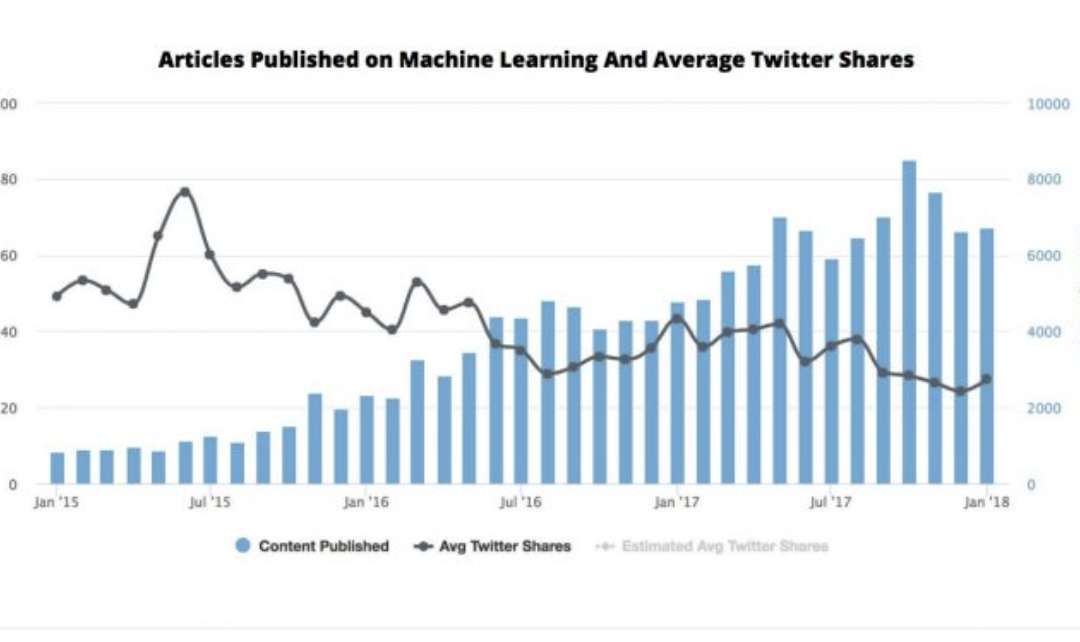
\includegraphics[scale=0.3]{figures/social-share-has-decreased.png}
    \centering
    \caption{Η δημοσιεύσεις κοινωνικών γεγονότων έχουν υποχωρήσει αισθητά. (Πηγή: \cite{[VEN+18]})}
    \label{socialsharing}
\end{figure}


Προκειμένου να επαναπροσδιοριστεί ο ρόλος των εφαρμογών, είναι απαραίτητο να αναθεωρηθούν τα κίνητρα με τα οποία αυτές κεντρίζουν το ενδιαφέρον του χρήστη. Η κοινωνική επίδειξη, να αντικατασταθεί με την κοινωνική συνεισφορά, ενώ η απομόνωση θα πρέπει να δώσει τη θέση της στην επανένταξη του ατόμου στο κοινωνικό σύνολο. Η ενημέρωση μέσω των εφαρμογών, οφείλει να έχει κοινωνικό χαρακτήρα και όχι να προβάλλει την προσωπική ζωή, ή να ωθεί σε κοινωνικά σύνδρομα τους χρήστες \cite{[BBC+18]}. 

\subsection{Ανάγκη της Κοινωνικής Προσφοράς}
Έχοντας υπόψη τα παραπάνω, καταλήγει κανείς εύκολα στο συμπέρασμα ότι υπάρχει μεγάλη ανάγκη να επανασυνδεθεί ο ρόλος των κοινωνικών εφαρμογών με την συνεισφορά για το κοινό συμφέρον. Αν και ζούμε σε μία εποχή όπου η τεχνολογία προχωράει με αλματώδεις ρυθμούς, ελάχιστο είναι το ποσοστό του συνόλου που γνωρίζει για τα επιτεύγματα των συγχρόνων του στους διάφορους επιστημονικόυς τομείς. Ακόμη κι αν το άτομο εκδηλώνει ενδιαφέρον, είναι δύσκολο να ενημερωθεί όταν όλες οι θεματικές περιστρέφονται γύρω από την προσωπική ζωή. Προκύπτει, λοιπόν μια νέα ανάγκη για κινητοποίηση του χρήστη να αλληλεπιδράσει με το κοινωνικό σύνολο. Αυτό είναι εφικτό χρησιμοποιώντας τις δυνατότητες των ήδη γνωστών εφαρμογών, αυτή τη φορά με σκοπό την ενημέρωση για γεγονότα που αφορούν την ευρύτερη πολιτισμική κοινότητα. 

\subsection{Η Έννοια του Πληθοπορισμού}
%Εδώ γράφουμε σύντομα τις τεχνικές/μεθοδολογίες/μοντέλα που πιθανά θα χρησιμοποιήσει η διπλωματική και είναι αναγκαία η κατανόησή τους από τον αναγνώστη πριν από την παρουσίαση της ανάλυσης και σχεδίασης του συστήματος. Πρόκειται για τεχνικές/μεθοδολογίες/μοντέλα που έχουν προταθεί από άλλους και δεν είναι πρωτότυπη δουλειά της διπλωματικής. Μετά βάζουμε μία ενότητα για κάθε τεχνική/μεθοδολογία/μοντέλο, όπου και δίνουμε λεπτομερή περιγραφή.
<<<<<<< HEAD
Συνδυάζοντας τη δύναμη της συλλογικής προσφοράς με την τεχνολογία και τεχνογνωσία που είναι διαθέσιμη σήμερα, η ενημέρωση μπορεί να πάρει νέα διάσταση. Με στοχευμένο προσανατολισμό της κοινωνικής διάθεσης για δράση προς μία συγκεκριμένη κατεύθυνση, η κοινωνία μπορεί να στρατολογήσει τα ίδια τα μέλη της προκειμένου να προάγει τις τεχνολογικές, πολιτισμικές και κοινωνικές εκδηλώσεις, να συντονίσει την πληροφορία και να ενημερώσει το σύνολο. Σύμφωνα με τη \selectlanguage{english}\textit{New York Times}\selectlanguage{greek}, χάρις στην αυξανόμενη συνδεσιμότητα μέσω του διαδικτύου, εκατομμύρια ανθρώπων μπορούν να συνεισφέρουν ιδέες και πληροφορίες για προβλήματα οποιασδήποτε μορφής. Η πρακτική της συμμετοχής ενός «πλήθους» ή μιας ομάδας για έναν κοινο στόχο ή επίλυση κοινών προβλημάτων, με την επιστράτευση της τεχνολογίας ως διαύλου επικοινωνίας ονομάζεται \textit{πληθοπορισμός} (\selectlanguage{english}\textit{crowdsourcing})\selectlanguage{greek} \cite{[CSW+18]}.
=======
Συνδυάζοντας τη δύναμη της συλλογικής προσφοράς με την τεχνολογία και τεχνογνωσία που είναι διαθέσιμη σήμερα, η ενημέρωση μπορεί να πάρει νέα διάσταση. Με στοχευμένο προσανατολισμό της κοινωνικής διάθεσης για δράση προς μία συγκεκριμένη κατεύθυνση, η κοινωνία μπορεί να στρατολογήσει τα ίδια τα μέλη της προκειμένου να προάγει τις τεχνολογικές, πολιτισμικές και κοινωνικές εκδηλώσεις, να συντονίσει την πληροφορία και να ενημερώσει το σύνολο. Σύμφωνα με τη \selectlanguage{english}\textit{New York Times}\selectlanguage{greek}, χάρις στην αυξανόμενη συνδεσιμότητα μέσω του διαδικτύου, εκατομμύρια ανθρώπων μπορούν να συνεισφέρουν ιδέες και πληροφορίες για προβλήματα οποιασδήποτε μορφής. Η πρακτική της συμμετοχής ενός «πλήθους» ή μιας ομάδας για έναν κοινο στόχο ή επίλυση κοινών προβλημάτων, με την επιστράτευση της τεχνολογίας ως διαύλου επικοινωνίας ονομάζεται \textit{πληθοπορισμός} (\selectlanguage{english}\textit{Crowdsourcing})\selectlanguage{greek} \cite{[CSW+18]}.
>>>>>>> acacc83a12cc6f1be99d6d3fb0df8b0ed3fa708b

\subsubsection{Εφαρμογές του Πληθοπορισμού}
Τα πεδία στα οποία μπορεί να αξιοποιηθεί η τεχνική του πληθοποριμού είναι αμέτρητα. Ο,τιδήποτε μπορεί να αποκτήσει συνεργατικό χαρακτήρα. Αναφορικά, παρατίθενται μερικοί κλάδοι όπου ανθεί η τεχνική αυτή:
\begin{description}[font=$\bullet$~\normalfont\color{black}]
\item [Εκπαίδευση]
\item [Οικονομία]
\item [Επιστήμη και Υγεία]
\item [ΙΤ]
\item [Διαφήμιση]
\item [Επιχειρηματικότητα]
<<<<<<< HEAD
\item [Κοινωνικές Εκδηλώσεις και \selectlanguage{english}\textit{NGO}\selectlanguage{greek}]
=======
\item [Κοινωνικές Εκδηλώσεις και ΜΚΟ]
>>>>>>> acacc83a12cc6f1be99d6d3fb0df8b0ed3fa708b
\end{description}

\subsubsection{Μοντέλο Πληθοπορισμού στην Εφαρμογή}
Η εφαρμογή σκοπεύει να χρησιμοποιήσει την πρακτική του πληθοπορισμού για να συγκεντρώσει πληροφορίες σχετικές με πολιτισμικές και κοινωνικές εκδηλώσεις. Οι χρήστες θα έχουν τη δυνατότητα να αξιολογούν τα πάντα γύρω από ένα γεγονός. Θα είναι δυνατή η ενημέρωση για τυχόν αλλαγές της ώρας και του τόπου, για προβλήματα που μπορεί να δυσκολέψουν την διεξαγωγή της εκδήλωσης, ή ιδέες για την καλυτέρευση αυτής. Το σημαντικό στοιχείο όλων των παραπάνω είναι πως θα μπορούν να γίνουν σε πραγματικό χρόνο. Αυτό θα έχει σαν αποτέλεσμα την καλύτερη αλληλεπίδραση μεταξύ συμμετεχόντων και διοργανωτών, την αποφυγή προβλημάτων και παρανοήσεων και την καλύτερη ενημέρωση του πλήθους. Διοργανωτές και συμμετέχοντες, θα μπορούν να εκφράσουν τη γνώμη τους, όλοι ως χρήστες της εφαρμογής. Η πληροφορία θα επικαιροποιείται διαρκώς από όσους παρευρίσκονται ήδη εκεί και θα διαδίδεται σε όσους μέχρι τώρα την αγνοούσαν.Το παραπάνω μοντέλο υλοποιειται μέσω ενός συστήματος μηνυμάτων μεταξύ των χρηστών. 

\section{Σχετικές Ερευνητικές Προσπάθειες και Πρότυπα}
Αν και το παρόν έργο αποτελεί προσωπική πρωτοβουλία, η ιδέα της διπλωματικής έχει κάποιες επιρροές και από άλλα παράλληλα έργα στον ίδιο τομέα. Τέτοια έργα είναι το \selectlanguage{english}\textit{WITHcrowd}\selectlanguage{greek} της ερευνητικής ομάδας του εργαστηρίου Ευφυών Συστημάτων (\selectlanguage{english}\textit{ISLAB}\selectlanguage{greek}) του Εθνικού Μετσόβιου  Πολυτεχνείου, που αποτελεί μέρος του ευρωπαϊκού προγράμματος \selectlanguage{english}\textit{WITH}\selectlanguage{greek}. Το έργο αυτό αποτέλεσε πηγή έμπνευσης για το κομμάτι του πληθοπορισμού στην εφαρμογή της παρούσας εργασίας. Χρησιμοποιήθηκαν επίσης to πρότυπo ανοιχού κώδικα \selectlanguage{english}\textit{Foursquare API}\selectlanguage{greek}, και οι διεπαφές αυτού,  \selectlanguage{english}\textit{Foursquare Autocomplete}\selectlanguage{greek} και \selectlanguage{english}\textit{Foursquare Places}\selectlanguage{greek}. Συνολικά, η εφαρμογή είναι μια καινοτομία η οποία προσπαθεί να στρέψει ήδη υπάρχουσες πρακτικές προς μια νέα κατεύθυνση, χρησιμοποιώντας τις σύγχρονη τεχνογνωσία για έναν πρωτοποριακό σκοπό.   

\subsection{\selectlanguage{english}WITHcrowd}
<<<<<<< HEAD
To \selectlanguage{english}WITHcrowd \cite{[WIT+18]}\selectlanguage{greek} είναι μια πρωτοβουλία της ευρωπαϊκής κοινότητας για τη συλλογή και ταξινόμηση δεδομένων πολιτισμικού περιεχομένου. Αποτελείται από μία πλατφόρμα που εκθέτει τις διεπαφές (ΑΡΙ) διαφόρων πυλών (\selectlanguage{english}portals)\selectlanguage{greek} και ψηφιακών αποθηκών (\selectlanguage{english}repositories)\selectlanguage{greek}. Eπιτρέπει στους χρήστες την αναζήτηση ψηφιακού περιεχομένου από μια σειρά διαφορετικών και ανεξάρτητων αποθετηρίων και βάσεων δεδομένων από ένα ενιαίο σημείο πρόσβασης. Τα αποθετήρια που μπορούν να αναζητηθούν περιλαμβάνουν μεταξύ άλλων την \selectlanguage{english}Europeana,\selectlanguage{greek} την Ψηφιακή Δημόσια Βιβλιοθήκη της Αμερικής, το \selectlanguage{english}YouTube,\selectlanguage{greek} το Μουσείο \selectlanguage{english}Rijks,\selectlanguage{greek} την Εθνική Βιβλιοθήκη της Αυστραλίας και την Ψηφιακή Νέα Ζηλανδία. Όλη η δύναμη της πλατφόρμας συγκεντρώνεται στο γεγονός ότι ο χρήστης είναι υπεύθυνος για την επίτευξη του στόχου του προγράμματος. Αυτή την πρακτική επιχειρεί να υιοθετήσει η εφαρμογή που θα αναλυθεί στα επόμενα κεφάλαια. 

\subsection{\selectlanguage{english}Foursquare API}
Το \selectlanguage{english}\textit{Foursquare API} \cite{[4SQ+18]}\selectlanguage{greek} είναι η διεπαφή της εφαρμογής \selectlanguage{english}\textit{Foursquare}\selectlanguage{greek} και παρέχεται στην κοινότητα της πληροφορικής δωρεάν. Δίνει τη δυνατότητα στους προγραμματιστές να χρησιμοποιήσουν δεδομένα που αφορούν τελικά σημεία (\selectlanguage{english}endpoints)\selectlanguage{greek} σε Ενιαίους Εντοπιστές Πόρων (\selectlanguage{english}URLs)\selectlanguage{greek}, όπως τα στοιχεία μιας υπηρεσίας (πχ. τοποθεσία, πληροφορίες επικοινωνίας, διεύθυνση, όνομα, κατηγορία, ώρες λειτουργίας, παροχές κλπ).
=======
To \selectlanguage{english}WITHcrowd\cite{[WIT+18]}\selectlanguage{greek} είναι μια πρωτοβουλία της ευρωπαϊκής κοινότητας για τη συλλογή και ταξινόμηση δεδομένων πολιτισμικού περιεχομένου. Αποτελείται από μία πλατφόρμα που εκθέτει τις διεπαφές (ΑΡΙ) διαφόρων πυλών (\selectlanguage{english}portals)\selectlanguage{greek} και ψηφιακών αποθηκών (\selectlanguage{english}repositories)\selectlanguage{greek}. Eπιτρέπει στους χρήστες την αναζήτηση ψηφιακού περιεχομένου από μια σειρά διαφορετικών και ανεξάρτητων αποθετηρίων και βάσεων δεδομένων από ένα ενιαίο σημείο πρόσβασης. Τα αποθετήρια που μπορούν να αναζητηθούν περιλαμβάνουν μεταξύ άλλων την \selectlanguage{english}Europeana,\selectlanguage{greek} την Ψηφιακή Δημόσια Βιβλιοθήκη της Αμερικής, το \selectlanguage{english}YouTube,\selectlanguage{greek} το Μουσείο \selectlanguage{english}Rijks,\selectlanguage{greek} την Εθνική Βιβλιοθήκη της Αυστραλίας και την Ψηφιακή Νέα Ζηλανδία. Όλη η δύναμη της πλατφόρμας συγκεντρώνεται στο γεγονός ότι ο χρήστης είναι υπεύθυνος για την επίτευξη του στόχου του προγράμματος. Αυτή την πρακτική επιχειρεί να υιοθετήσει η εφαρμογή που θα αναλυθεί στα επόμενα κεφάλαια. 

\subsection{\selectlanguage{english}Foursquare API}
Το \selectlanguage{english}\textit{Foursquare API}\cite{[4SQ+18]}\selectlanguage{greek} είναι η διεπαφή της εφαρμογής \selectlanguage{english}\textit{Foursquare}\selectlanguage{greek} και παρέχεται στην κοινότητα της πληροφορικής δωρεάν. Δίνει τη δυνατότητα στους προγραμματιστές να χρησιμοποιήσουν δεδομένα που αφορούν τελικά σημεία (\selectlanguage{english}endpoints)\selectlanguage{greek} σε Ενιαίους Εντοπιστές Πόρων (\selectlanguage{english}URLs)\selectlanguage{greek}, όπως τα στοιχεία μιας υπηρεσίας (πχ. τοποθεσία, πληροφορίες επικοινωνίας, διεύθυνση, όνομα, κατηγορία, ώρες λειτουργίας, παροχές κλπ).
>>>>>>> acacc83a12cc6f1be99d6d3fb0df8b0ed3fa708b

To \selectlanguage{english}\textit{Foursquare}\selectlanguage{greek} έφερε την επανάσταση στα μέσα κοινωνικής δικτύωσης με την καινοτομία του ``\textit{\selectlanguage{english}check in}''.  Η λειτουργία της εφαρμογής \selectlanguage{english}Foursquare\selectlanguage{greek} συνοψίζεται στην αξιολόγηση και άσκηση κριτικής σε κέντρα διασκέδασης, εστιατόρια και χώρους ψυχαγωγίας. Ο χρήστης δημοσιεύει την τοποθεσία του κάνοντας \selectlanguage{english}check in\selectlanguage{greek} και ενημερώνει τους υπόλοιπους χρήστες-φίλους του. Η εφαρμογή που θα υλοποιηθεί κάνει μια απόπειρα να διοχετεύσει την πληροφορία σε αντίστοιχα μέρη πολιτισμικού ή κοινωνικού περιεχομένου και να την αξιοποιήσει για την αξιολόγησή τους.


\section{\selectlanguage{greek}Τεχνολογικό υπόβαθρο - Βασικές Έννοιες}
Στη συνέχεια θα γίνει μια εισαγωγή στις τεχνολογίες και τα εργαλεία προγραμματισμού. Έπειτα ακολουθεί η ανάλυση των σύγχρονων τεχνολογικών μέσων που αποτελούν τη βάση των μεθόδων και μοντέλων που χρησιμοποιήθηκαν στην υλοποίηση της εφαρμογής. 

Όταν ένας προγραμματιστής αναπτύσσει μία εφαρμογή, καλείται να προσδιορίσει τρία πράγματα:
\begin{enumerate}
\item Tην φύση της εφαρμογής - αν θα τρέχει σε φυλλομετρητή (\selectlanguage{english}Web Application)\selectlanguage{greek} ή αν θα είναι μητρική (\selectlanguage{english}Native Application)\selectlanguage{greek}.
\item Την γλώσσα στην οποία θα αναπτύξει την εφαρμογή (\selectlanguage{english}Programming Language)\selectlanguage{greek}
\item Την πλατφόρμα λογισμικού στην οποία θα υλοποιήσει την εφαρμογή (\selectlanguage{english}\textit{SDK})\selectlanguage{greek}
\end{enumerate}

\subsection{Είδη Γλωσσών Προγραμματισμού}
Πρωτού μιλήσουμε για τα είδη των σύγχρονων εφαρμογών, είναι απαραίτητο να αναλύσουμε τις κατηγορίες των αντίστοιχων γλωσσών και τις διακρίσεις μεταξύ αυτών. Μια γλώσσα μπορεί να ανήκει σε μία από τις παρακάτω κατηγορίες:
\begin{description}[font=$\bullet$~\normalfont\color{black}]
\item [Μετταγλωτισμένες ή Μητρικές γλώσσες (\selectlanguage{english}Compiled or Native Languages)]\selectlanguage{greek}
\item [Διαχειριζόμενες Γλώσσες (\selectlanguage{english}Managed Languages)]\selectlanguage{greek}
\item [Δυναμικές Γλώσσες (\selectlanguage{english}Dynamic Languages)]\selectlanguage{greek}
<<<<<<< HEAD
\end{description}Η μητρική γλώσσα (\selectlanguage{english}native language)\selectlanguage{greek} είναι μια γλώσσα που μπορεί να τρέξει στην πλατφόρμα του λειτουργικού συστήματος χωρίς να μετατραπεί σε άλλη μορφή κώδικα από τους μεταγλωττιστές (\selectlanguage{english}compilers)\selectlanguage{greek}. Αυτό σημαίνει πως η υλοποίησή της συνοψίζεται κυρίως στη χρήση μεταγλωττιστών, οι οποίοι είναι υπεύθυνοι για τη μετατροπή του κώδικα από γλώσσα μηχανής σε πηγαίο κώδικα (πχ. \selectlanguage{english}\textit{C++, C\#, Java, Swift})\selectlanguage{greek}. Η διαχειριζόμενη γλώσσα (\selectlanguage{english}managed language)\selectlanguage{greek} είναι μια γλώσσα που πρέπει να μετατραπεί ή να ερμηνευτεί πριν να εκτελεστεί στην πλατφόρμα (πχ.\selectlanguage{english} \textit{.NET})\selectlanguage{greek}. Σε αυτή την περίπτωση, ο κώδικας θα εκτελεστεί υπό τη διαχείριση μιας εικονικής μηχανής γλώσσας κοινού χρόνου εκτέλεσης ή, όπως είναι γνωστή,\selectlanguage{english} \textit{CLR}\selectlanguage{greek} \cite{[STR+09],[DEV+03]} (βλ. Σχ. \ref{clr}). Η δυναμική γλώσσα προγραμματισμού (\selectlanguage{english}dynamic language)\selectlanguage{greek} είναι μια κλάση αποτελούμενη από γλώσσες υψηλού επιπέδου (\selectlanguage{english}high-level programming languages)\selectlanguage{greek}, οι οποίες έχουν την ιδιότητα να εκτελούν πολλαπλές εντολές κατά το στάδιο της εκτέλεσης, σε αντίθεση με τις υπόλοιπες γλώσσες που εκτελούν εντολές στο στάδιο μεταγλώττισης  (πχ.\selectlanguage{english} \textit{Python, JavaScript, PHP, Ruby, MATLAB, Elixir})\selectlanguage{greek} \cite{[MIC05], [ADV09]}.

\begin{figure}[H]
    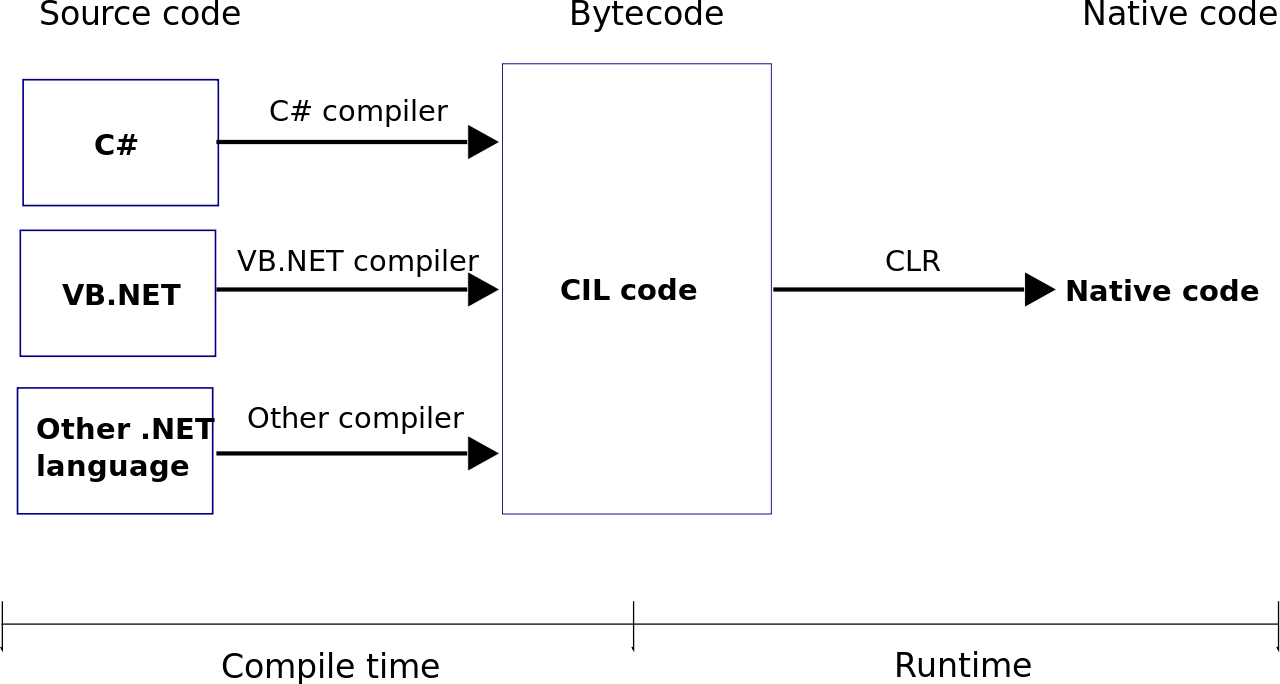
\includegraphics[scale=0.3]{figures/clr-converts-language-to-native-code.png}
    \centering
    \caption{Το \selectlanguage{english}CLR\selectlanguage{greek} μετατρέπει \selectlanguage{english}CIL\selectlanguage{greek} σε μητρικό κώδικα.}
    \label{clr}
\end{figure}
=======
\end{description}Η μητρική γλώσσα (\selectlanguage{english}native language)\selectlanguage{greek} είναι μια γλώσσα που μπορεί να τρέξει στην πλατφόρμα του λειτουργικού συστήματος χωρίς να μετατραπεί σε άλλη μορφή κώδικα από τους μεταγλωττιστές (\selectlanguage{english}compilers)\selectlanguage{greek}. Αυτό σημαίνει πως η υλοποίησή της συνοψίζεται κυρίως στη χρήση μεταγλωττιστών (\selectlanguage{english}compilers)\selectlanguage{greek}, οι οποίοι είναι υπεύθυνοι για τη μετατροπή του κώδικα από γλώσσα μηχανής σε πηγαίο κώδικα (πχ. \selectlanguage{english}\textit{C++, C\#, Java, Swift})\selectlanguage{greek}. Η διαχειριζόμενη γλώσσα (\selectlanguage{english}managed language)\selectlanguage{greek} είναι μια γλώσσα που πρέπει να μετατραπεί ή να ερμηνευτεί πριν να εκτελεστεί στην πλατφόρμα (πχ.\selectlanguage{english} \textit{.NET})\selectlanguage{greek}. Σε αυτή την περίπτωση, ο κώδικας θα εκτελεστεί υπό τη διαχείριση μιας εικονικής μηχανής γλώσσας κοινού χρόνου εκτέλεσης ή, όπως είναι γνωστή,\selectlanguage{english} \textit{CLR}\selectlanguage{greek} \cite{[STR+09],[DEV+03]}. Η δυναμική γλώσσα προγραμματισμού (\selectlanguage{english}dynamic language)\selectlanguage{greek} είναι μια κλάση αποτελούμενη από γλώσσες υψηλού επιπέδου (\selectlanguage{english}high-level programming languages)\selectlanguage{greek}, οι οποίες έχουν την ιδιότητα να εκτελούν πολλαπλές εντολές κατά το στάδιο της εκτέλεσης, σε αντίθεση με τις υπόλοιπες γλώσσες που εκτελούν εντολές στο στάδιο μεταγλώττισης  (πχ.\selectlanguage{english} \textit{Python, JavaScript, PHP, Ruby, MATLAB, Elixir})\selectlanguage{greek} \cite{[MIC05], [ADV09]}.
>>>>>>> acacc83a12cc6f1be99d6d3fb0df8b0ed3fa708b

Οι γλώσσες υψηλού επιπέδου, όπως η \selectlanguage{english}Python\selectlanguage{greek} και η \selectlanguage{english}Ruby\selectlanguage{greek}, έχουν αποκτήσει μεγάλη απήχηση τα τελευταία χρόνια. Για πολλούς, αποτελούν τη νέα γεννιά γλωσσών προγραμματισμού. Ωστόσο οι ρίζες τους ανατρέχουν στις αρχές της δεκαετίας του '50, με την γέννηση της \selectlanguage{english}Lisp\selectlanguage{greek} της πρώτης γλώσσας υψηλού επιπέδου. Πλέον, οι δυναμικές γλώσσες συναντόνται τόσο σε πραγματικά διαδικτυακά συστήματα, όσο και σε εφαρμογές που πριν κυριαρχούσαν οι στατικές γλώσσες προγραμματισμού \cite{[ADV09]}.

Εμείς θα επικεντρωθούμε στην πρώτη κατηγορία, των μητρικών ή αλλιώς μεταφρασμένων γλωσσών προγραμματισμού. Το πλεονέκτημα χρήσης μητρικού κώδικα (\selectlanguage{english}native code\selectlanguage{greek}) βρίσκεται στο γεγονός ότι προγράμματα σε τέτοιες γλώσσες είναι γρηγορότερα, χάρις τον μειωμένο χρόνο επιβάρυνσης (\selectlanguage{english}overhead)\selectlanguage{greek} της διαδικασίας μετάφρασης. Αυτό οφείλεται στην ιδιότητά τους να μεταγλωττίζονται κατά το χρόνο μεταγλώττισης και όχι κατά το χρόνο εκτέλεσης, όπως συμβαίνει με άλλα προγράμματα.

Οι γλώσσες χαμηλού επιπέδου (\selectlanguage{english}low-level programming languages)\selectlanguage{greek} είναι δομημένες έτσι ώστε να υφίστανται την τυπική μεταγλώττιση, ειδικά όταν η αποτελεσματικότητα είναι πρωταρχικό μέλημα, έναντι της μεταγλώττισης που υποστηρίζει πολλές πλατφόρμες (\selectlanguage{english}cross-platform)\selectlanguage{greek}. Για αυτές τις γλώσσες, υπάρχουν περισσότερες ένα-προς-ένα αντιστοιχίες ανάμεσα στο προγραμματισμένο κώδικα και τις λειτουργίες υλικού που εκτελούνται σε κώδικα μηχανής, καθιστώντας ευκολότερο για τους προγραμματιστές τον έλεγχο χρήσης της κεντρικής μονάδας επεξεργασίας και μνήμης με λεπτομέρεια. 
<<<<<<< HEAD
Με κάποια προσπάθεια, είναι πάντα δυνατή η σύνταξη μεταγλωττιστών ακόμα και για παραδοσιακά ερμηνευμένες γλώσσες. Για παράδειγμα, η\selectlanguage{english} Common lisp\selectlanguage{greek} μπορεί να μεταγλωττιστεί σε \selectlanguage{english}Java bytecode\selectlanguage{greek} (στη συνέχεια ερμηνεύεται από την εικονική μηχανή\selectlanguage{english} Java\selectlanguage{greek}), σε κώδικα\selectlanguage{english} C\selectlanguage{greek} (στη συνέχεια, μεταγλωττίζεται στον εγγενή κώδικα μηχανής) ή απευθείας σε εγγενή κώδικα. Οι γλώσσες προγραμματισμού που υποστηρίζουν πολλαπλούς στόχους σύνταξης δίνουν μεγαλύτερο έλεγχο στους προγραμματιστές για να επιλέξουν είτε ταχύτητα εκτέλεσης είτε συμβατότητα μεταξύ πολλαπλών πλατφόρμων \cite{[SQA+07]}.

\clearpage
=======
Με κάποια προσπάθεια, είναι πάντα δυνατή η σύνταξη μεταγλωττιστών ακόμα και για παραδοσιακά ερμηνευμένες γλώσσες. Για παράδειγμα, η\selectlanguage{english} Common lisp\selectlanguage{greek} μπορεί να μεταγλωττιστεί σε \selectlanguage{english}Java bytecode\selectlanguage{greek} (στη συνέχεια ερμηνεύεται από την εικονική μηχανή\selectlanguage{english} Java\selectlanguage{greek}), σε κώδικα\selectlanguage{english} C\selectlanguage{greek} (στη συνέχεια, μεταγλωττίζεται στον εγγενή κώδικα μηχανής) ή απευθείας σε εγγενή κώδικα. Οι γλώσσες προγραμματισμού που υποστηρίζουν πολλαπλούς στόχους σύνταξης δίνουν μεγαλύτερο έλεγχο στους προγραμματιστές για να επιλέξουν είτε ταχύτητα εκτέλεσης είτε συμβατότητα μεταξύ πλατφόρμων \cite{[SQA+07]}.
>>>>>>> acacc83a12cc6f1be99d6d3fb0df8b0ed3fa708b

\selectlanguage{english}
\begin{lstlisting}[language=Python, caption=\selectlanguage{greek}Παράδειγμα κώδικα σε \selectlanguage{english}Python]
import numpy as np
 
def incmatrix(genl1,genl2):
    m = len(genl1)
    n = len(genl2)
    M = None #to become the incidence matrix
    VT = np.zeros((n*m,1), int)  #dummy variable
 
    #compute the bitwise xor matrix
    M1 = bitxormatrix(genl1)
    M2 = np.triu(bitxormatrix(genl2),1) 
 
    for i in range(m-1):
        for j in range(i+1, m):
            [r,c] = np.where(M2 == M1[i,j])
            for k in range(len(r)):
                VT[(i)*n + r[k]] = 1;
                VT[(i)*n + c[k]] = 1;
                VT[(j)*n + r[k]] = 1;
                VT[(j)*n + c[k]] = 1;
 
                if M is None:
                    M = np.copy(VT)
                else:
                    M = np.concatenate((M, VT), 1)
 
                VT = np.zeros((n*m,1), int)
 
    return M
\end{lstlisting}

\selectlanguage{greek}
\subsection{Μητρικές Γλώσσες Προγραμματισμού (\selectlanguage{english}Native Programming Languages)}
\selectlanguage{greek}
%Μιλάμε για τις δυνατοτητες τους και τα μειονεκτηματα τους (αναφορα σε σχετικα αρθρα, παραθεση δειγματος κωδικα και παραθεση διαγραμματων με την πτωση της χρησης τους)
Έχοντας προσδιορίσει τις κατηγορίες γλωσσών προγραμματισμού, μπορεί κανείς επομένως να αντιληφθεί την ανάγκη των μητρικών ή αλλιώς μεταγλωττισμένων γλωσσών για την ανάπτυξη εφαρμογών σε συγκεκριμένες πλατφόρμες. Αυτές οι γλώσσες είναι κατά κύριο λόγο σχεδιασμένες να τρέχουν σε μια ορισμένη πλατφόρμα για καλύτερη απόδοση και ευκολότερο σχεδιασμό. Τέτοιες γλώσσες που χρησιμοποιούνται σήμερα στις εφαρμογές κινητών συσκευών είναι η \selectlanguage{english}Swift\selectlanguage{greek} και η \selectlanguage{english}Java\selectlanguage{greek}. Η πρώτη χρησιμοποιείται για την υλοποίηση εφαρμογών σε \selectlanguage{english}iOS\selectlanguage{greek} πλατφόρμες, ενώ η δεύτερη για την ανάπτυξη εφαρμογών που τρέχουν σε \selectlanguage{english}Android\selectlanguage{greek} πλατφόρμες.

\subsubsection{\selectlanguage{english}Swift - iOS Development}
\selectlanguage{greek}
Η \selectlanguage{english}\textit{Swift}\selectlanguage{greek} είναι μια μεταγλωττισμένη, γενικού σκοπού, πολυπαραδειγματική γλώσσα προγραμματισμού που έχει αναπτυχθεί από την \selectlanguage{english}\textit{Apple Inc.}\selectlanguage{greek} για τα προϊόντα τις ίδιας εταιρείας (\selectlanguage{english}\textit{iOS, macOS, watchOS, tvOS}\selectlanguage{greek}). Είναι σχεδιασμένη ώστε να δουλεύει με το \textit{\selectlanguage{english}XCode IDE\selectlanguage{greek}} και χρησιμοποιείται από την κοινότητα των \selectlanguage{english}iOS developers\selectlanguage{greek} για ανάπτυξη \selectlanguage{english}iOS\selectlanguage{greek} εφαρμογών, υποστηριζόμενων από τις πλατφόρμες και τα προϊόντα \selectlanguage{english}Apple\selectlanguage{greek} \cite{[SWIFT1+16]}.

Τα πρώτα βήματα για την δημιουργία της \selectlanguage{english}Swift\selectlanguage{greek} ξεκίνησαν υπό την καθοδήγηση του \selectlanguage{english}C.~Lattner\selectlanguage{greek}, εντός της \selectlanguage{english}Apple\selectlanguage{greek}. Με επιρροές από γλώσσες όπως οι \selectlanguage{english}\textit{Objective-C, Rust, Haskell, C\#}\selectlanguage{greek} και αρκετές ακόμη \cite{[SWIFT2+14]}, η \selectlanguage{english}Swift\selectlanguage{greek} ήρθε στο προσκήνιο επίσημα για πρώτη φορά στο Παγκόσμιο Συνέδριο Προγραμματιστών (\selectlanguage{english}WWDC\selectlanguage{greek}) τον Ιούνιο του 2014 \cite{[SWIFT3+14]}. 

Βασικά γνωρίσματα αυτής της γλώσσας είναι η αντικειμενοστρέφεια (\selectlanguage{english}\textit{OO} language\selectlanguage{greek}), και η απλουστευμένες δομές. Η \selectlanguage{english}Swift\selectlanguage{greek} βασίζεται σε θεωρητικές έννοιες των μοντέρνων γλωσσών προγραμματισμού και προσπαθεί να παρουσιάσει μια απλούστερη συντακτική προσέγγιση \cite{[SWIFT4], [SWIFT5]}. 

\selectlanguage{english}
\begin{lstlisting}[language=Swift, caption=\selectlanguage{greek}Παράδειγμα κώδικα σε \selectlanguage{english}Swift]
    import UIKit
    import AVFoundation
    
class ViewController: UIViewController {
    
    @IBOutlet weak var darkBlueBG: UIImageView!
    @IBOutlet weak var powerBtn: UIButton!
    @IBOutlet weak var cloudHolder: UIView!
    @IBOutlet weak var rocket: UIImageView!
    @IBOutlet weak var hustleLbl: UILabel!
    @IBOutlet weak var onLbl: UILabel!
    
    var player: AVAudioPlayer!
    
    override func viewDidLoad() {
        super.viewDidLoad()
        
        let path = Bundle.main.path(forResource: "hustle-on", ofType: "wav")!
        let url = URL(fileURLWithPath: path)
        do {
            player = try AVAudioPlayer(contentsOf: url)
            player.prepareToPlay()
        } catch let error as NSError {
            print(error.description)
        }
    }
    
    @IBAction func powerBtnPressed(_ sender: Any) {
        cloudHolder.isHidden = false
        darkBlueBG.isHidden = true
        powerBtn.isHidden = true
        
        player.play()
        
        UIView.animate(withDuration: 2.3, animations: {
            self.rocket.frame = CGRect(x: 0, y: 140, width: 375, height: 402)
        }) { (finished) in
            self.hustleLbl.isHidden = false
            self.onLbl.isHidden = false
        }
    }
}

\end{lstlisting}


\subsubsection{\selectlanguage{english}Java - Android Development}
\selectlanguage{greek}
Η \selectlanguage{english}\textit{Java}\selectlanguage{greek} είναι γενικού σκοπού, ταυτοχρονισμένη (\selectlanguage{english}concurrent\selectlanguage{greek}), βασισμένη σε κλάσεις (\selectlanguage{english}class-based\selectlanguage{greek}) και αντικειμενοστραφής (\selectlanguage{english}\textit{OO}\selectlanguage{greek}) γλώσσα \cite{[JAVA1]}. Έχει σχεδιαστεί ειδικά για να επιτρέπει όσο το δυνατό μεγαλύτερη ανεξαρτησία στον προγραμματιστή και ευελιξία όσον αφορά τη συγγραφή κώδικα με συνδυασμό πολλών βιβλιοθηκών. Ακολουθεί τη νοοτροπία ``\selectlanguage{english}\textit{WORA}\selectlanguage{greek}'' \cite{[JAVA2]}, με αποτέλεσμα να μπορεί να τρέξει σε όλες τις πλατφόρμες που υποστηρίζουν \selectlanguage{english}Java\selectlanguage{greek} χωρις να χρείαζεται επαναμεταγλώττιση \cite{[JAVA3]}. Από το 2016 η \selectlanguage{english}Java\selectlanguage{greek} έχει ανέλθει σε μία από τις δημοφιλέστερες εν ενεργεία γλώσσες προγραμματισμού \cite{[JAVA4], [JAVA5], [JAVA6]}.

Η \selectlanguage{english}Java\selectlanguage{greek} εμφανίστηκε στο προσκήνιο το 1991, χάρις στον \selectlanguage{english}J. Gosling\selectlanguage{greek} και τους συνεργάτες του. Η πρώτη επίσημη δημοσίευση έγινε το 1996 από την εταιρεία \selectlanguage{english}Sun Microsystems\selectlanguage{greek} \cite{[JAVA8]}. Σύντομα, ενσωματώθηκε στους σημαντικότερους φυλλομετρητές ιστού (\selectlanguage{english}web browsers\selectlanguage{greek}), και σε ιστοσελίδες (\selectlanguage{english}web pages\selectlanguage{greek}), πράγμα που την μετέτρεψε σε ισχυρό προγραμματιστικό εργαλείο. Η \selectlanguage{english}Java\selectlanguage{greek} δέχθηκε αρκετές επιρροές από τη \selectlanguage{english}C++\selectlanguage{greek}, όσον αφορά το συντακτικό κομμάτι. Όντας επίσης μιας αντικειμενοσταφής γλώσσα προγραμματισμού, η \selectlanguage{english}Java\selectlanguage{greek} θεμελιώνεται σε κλάσεις (\selectlanguage{english}classes\selectlanguage{greek}) και κάθε ομάδα δεδομένων αποτελεί ένα ``\textit{αντικείμενο}'' (\selectlanguage{english}\textit{object}\selectlanguage{greek}). Εξαίρεση αποτελούν οι πρωτογενείς τύποι δεδομένων (πχ \selectlanguage{english}\textit{integers, floating points, boolean values}\selectlanguage{greek} κλπ)

To 2005, η \selectlanguage{english}Google\selectlanguage{greek} ανακοίνωσε ένα νέο λειτουργικό σύστημα προοριζόμενο για φορητές συσκευές με το όνομα \selectlanguage{english}Android\selectlanguage{greek}. Πρόκειται για μια παραλλαγή του πυρήνα του λειτουργικού συστήματος \selectlanguage{english}Linux\selectlanguage{greek}, με προσθήκες από κάποιες ακόμη βιβλιοθήκες ανοιχτού λογισμικού. Το λογισμικό \selectlanguage{english}Android\selectlanguage{greek} υποστηρίζεται από συσκευές 3ης γενιάς (\selectlanguage{english}smartphones, tablets\selectlanguage{greek}) καθώς και άλλα προϊόντα της \selectlanguage{english}Google\selectlanguage{greek} (πχ \selectlanguage{english}\textit{Android Auto, Android TV, Wear OS}\selectlanguage{greek} κλπ). οι εφαρμογές που αναπτύσσονται με αυτό το λειτουργικό σύστημα υλοποιούνται με τη χρήση της πλατφόρμας \selectlanguage{english}\textit{Android Studio SDK} \cite{[JAVA9]}\selectlanguage{greek} και της γλώσσας \selectlanguage{english}Java \cite{[JAVA10]}\selectlanguage{greek}. Την πλατφόρμα αυτή συνοδεύουν και άλλα χρήσιμα εργαλεία, όπως αποσφαλματωτής (\selectlanguage{english}debugger\selectlanguage{greek}), βιβλιοθήκες λογισμικού και προσομοιωτής (\selectlanguage{english}emulator\selectlanguage{greek}) \cite{[JAVA11]}.

\selectlanguage{english}
\begin{lstlisting}[language=Java, caption=\selectlanguage{greek}Παράδειγμα κώδικα σε \selectlanguage{english}Java]
// This is an example of a single line comment using two slashes

/* This is an example of a multiple line comment using the slash and asterisk.
 This type of comment can be used to hold a lot of information or deactivate
 code, but it is very important to remember to close the comment. */

package fibsandlies;
import java.util.HashMap;

/**
 * This is an example of a Javadoc comment; Javadoc can compile documentation
 * from this text. Javadoc comments must immediately precede the class, method, or field being documented.
 */
public class FibCalculator extends Fibonacci implements Calculator {

    private static Map<Integer, Integer> memoized = new HashMap<Integer, Integer>();

    /*
     * The main method written as follows is used by the JVM as a starting point for the program.
     */
    public static void main(String[] args) {
        memoized.put(1, 1);
        memoized.put(2, 1);
        System.out.println(fibonacci(12)); //Get the 12th Fibonacci number and print to console
    }

    /**
     * An example of a method written in Java, wrapped in a class.
     * Given a non-negative number FIBINDEX, returns
     * the Nth Fibonacci number, where N equals FIBINDEX.
     * @param fibIndex The index of the Fibonacci number
     * @return The Fibonacci number
     */
    public static int fibonacci(int fibIndex) {
        if (memoized.containsKey(fibIndex)) {
            return memoized.get(fibIndex);
        } else {
            int answer = fibonacci(fibIndex - 1) + fibonacci(fibIndex - 2);
            memoized.put(fibIndex, answer);
            return answer;
        }
    }
}
<<<<<<< HEAD
\end{lstlisting}



\subsection{\selectlanguage{english}JavaScript in Mobile Applications}
\selectlanguage{greek}
% Μιλαμε εισαγωγικα για τη γλωσσα αυτη, ιδεες απο τη διπλωματικη του παιδιου και περναμε στην Ρεακτ. Μιλαμε για τα γνωρισματα και τα πλεονεκτηματα της (παρε την περιληψη που εγραψες).
H \selectlanguage{english}\textit{JavaScript}\selectlanguage{greek}, γνωστή και με την ακρωνυμία \selectlanguage{english}\textit{JS}\selectlanguage{greek}, είναι μία γλώσσα υψηλού επιπέδου, που ανήκει στην κατηγορία των μεταγλωττισμένων γλωσσών προγραμματισμού. Συμμορφώνεται στους διακονινισμoύς που ορίζονται από το πρότυπο \selectlanguage{english}\textit{ES}\selectlanguage{greek} \cite{[JS1]}. Χρησιμοποιείται κυρίως στον \selectlanguage{english}client-side\selectlanguage{greek} προγραμματρισμό, αποτελόντας τον πυρήνα των τεχνολογιών που χρησιμοποιούνται σήμερα στην πλειοψηφία των \selectlanguage{english}web\selectlanguage{greek} εφαρμογών και ιστοσελίδων \cite{[JS2]}. Σαν πολυπαραδειγματική γλώσσα, η  \selectlanguage{english}JavaScript\selectlanguage{greek} υποστηρίζει όλες τις σύχρονες τεχνικές προγραμματισμού, όπως συναρτησιακό \selectlanguage{english}(functional)\selectlanguage{greek}, οδηγούμενο από γεγονότα \selectlanguage{english}(event-driven)\selectlanguage{greek} και αντικειμενοστραφή \selectlanguage{english}(object-oriented)\selectlanguage{greek} προγραμματισμό. 

Από το Μάιο του 2017, το 94.5\% των δημοφιλέστερων ιστοσελίδων είναι γραμμένα σε \selectlanguage{english} JavaScript\selectlanguage{greek}. Η πιο συνηθισμένος τρόπος χρήσης της είναι για την ανάπτυξη προγραμμάτων-πελατών (\selectlanguage{english}clients\selectlanguage{greek}) που είναι γραμμένα σε τυπική \selectlanguage{english}HTML\selectlanguage{greek}. Το κυριότερο χαρακτηριστικό της είναι ότι προσδίδει κάποιες χρηστικές ιδιότητες στον καθιερωμένο κώδικα, που καθιστούν τα προγράμματα περισσότερο αποκρίσιμα, μέσω πληθώρας στοιχείων αλληλεπίδρασης με το \selectlanguage{english}\textit{DOM}\selectlanguage{greek}. Οι πιο κοινές περιπτώσεις αυτών είναι:  

\begin{itemize}
\item Η φόρτωση νέου περιεχομένου σελίδας ή η υποβολή δεδομένων στον διακομιστή μέσω του συστήματος \selectlanguage{english}\textit{AJAX}\selectlanguage{greek} χωρίς επαναφόρτωση της σελίδας (για παράδειγμα, ένα κοινωνικό δίκτυο ενδέχεται να επιτρέψει στο χρήστη να δημοσιεύει ενημερώσεις κατάστασης χωρίς να εγκαταλείψει τη σελίδα).
\item Κινούμενα σχέδια των στοιχείων της σελίδας, \selectlanguage{english}fade out/in, slide out/in,\selectlanguage{greek} αλλαγή μεγέθους, αποκοπή, μετακίνηση, κλπ.
\item Διαδραστικό περιεχόμενο, για παράδειγμα παιχνίδια, αναπαραγωγή ήχου και βίντεο.
\item Επαλήθευση των τιμών εισαγωγής μιας φόρμας διαδικτύου για επιβεβαίωση ότι είναι αποδεκτές πριν υποβληθεί στο διακομιστή.
\item Μετάδοση πληροφοριών σχετικά με τις συνήθειες ανάγνωσης του χρήστη και τις δραστηριότητες περιήγησης σε διάφορους ιστότοπους. Οι ιστοσελίδες το συνηθίζουν αυτό σε αναλύσεις στο \selectlanguage{english}Web\selectlanguage{greek}, για παρακολούθηση διαφημίσεων, εξατομίκευση ή για άλλους σκοπούς.
\end{itemize}

Τα παραπάνω επιτυγχάνονται πρακτικά με την ενσωμάτωση τμημάτων κώδικα (\selectlanguage{english}script objects\selectlanguage{greek}) γραμμένο σε \selectlanguage{english}JS\selectlanguage{greek}, εντός του κυρίου μέρους (\selectlanguage{english}body\selectlanguage{greek}) που είναι γραμμένο σε παραδοσιακή \selectlanguage{english}HTML\selectlanguage{greek}. Ένα πρόγραμμα περιήγησης στο \selectlanguage{english}web\selectlanguage{greek} είναι το πιο κοινό περιβάλλον υποδοχής για \selectlanguage{english}JavaScript\selectlanguage{greek}. Εκεί δημιουργούνται συνήθως ``\textit{αντικείμενα φιλοξενίας}'' (\selectlanguage{english}host objects\selectlanguage{greek}) για την αναπαράσταση του \selectlanguage{english}DOM\selectlanguage{greek}. Ο διακομιστής  \selectlanguage{english}Web (server\selectlanguage{greek}) είναι ένα άλλο κοινό περιβάλλον υποδοχής. Ένας \selectlanguage{english}Web JavaScript server\selectlanguage{greek} συνήθως εκθέτει αντικείμενα φιλοξενίας που αντιπροσωπεύουν αντικείμενα αιτήματος και απόκρισης \selectlanguage{english}HTTP (HTTP requests)\selectlanguage{greek}, τα οποία ένα πρόγραμμα σε \selectlanguage{english}JavaScript\selectlanguage{greek} θα μπορούσε στη συνέχεια να αξιολογήσει και να διαχειριστεί προκειμένου να δημιουργήσει δυναμικά ιστοσελίδες. 

\selectlanguage{english}
\begin{lstlisting}[language=HTML5, caption=\selectlanguage{greek}Μικρό παράδειγμα μιας ιστοσελίδας που συμμορφώνεται με τα πρότυπα και περιέχει \selectlanguage{english}JavaScript\selectlanguage{greek} (χρησιμοποιώντας τη σύνταξη \selectlanguage{english}HTML5\selectlanguage{greek}) και το \selectlanguage{english}DOM\selectlanguage{greek}]
<!DOCTYPE html>
<html>
  <head>
    <title>Example</title>
  </head>
  <body>
    <button id="hellobutton">Hello</button>
    <script>
        document.getElementById('hellobutton').onclick = function() {
            alert('Hello world!');  // Show a dialog
            var myTextNode = document.createTextNode('Some new words.');
            document.body.appendChild(myTextNode);  // Append "Some new words" to the page
        };
    </script>
  </body>
</html>
\end{lstlisting}
\selectlanguage{greek}

\subsubsection{Βρόχος Συμβάντων - \selectlanguage{english}Event Loop\selectlanguage{greek}}

Στη \selectlanguage{english}JavaScript\selectlanguage{greek}, σχεδόν όλες οι λειτουργίες εισόδου/εξόδου (I/O) εκτελούνται ασύγχρονα, χωρίς μπλοκάρισμα (\selectlanguage{english}non-blocking execution\selectlanguage{greek}). Σε αυτές περιλαμβάνονται \selectlanguage{english}HTTP\selectlanguage{greek} αιτήσεις, ενέργειες πάνω σε βάσεις δεδομένων, εγγραφές και αναγνώσεις από το σκληρό δίσκο. Το μοναδικό νήμα ζητά από το περιβάλλον εκτέλεσης να πραγματοποιήσει μια ενέργεια, παρέχοντάς του μια συνάρτηση επανάκλησης (\selectlanguage{english}callback function\selectlanguage{greek}), συνεχίζοντας με την εκτέλεση άλλων εργασιών. Όταν η ενέργεια που ζητήθηκε προηγουμένως ολοκληρωθεί, ένα μήνυμα εισάγεται σε μια ουρά μαζί με το παρεχόμενο ανάκλησης \selectlanguage{english}(callback content)\selectlanguage{greek}. Κάποια στιγμή στο μέλλον, το μήνυμα αυτό θα αφαιρεθεί από την ουρά και η συνάρτηση επανάκλησης θα εκτελεστεί. Αυτό το διαδραστικό, πλήρως ασύγχρονο, μοντέλο μπορεί να είναι γνώριμο στους προγραμματιστές που
αναπτύσσουν λογισμικό διεπαφής χρήστη (ΑΡΙ) \textit{\textbf{--}} εκεί που συμβάντα όπως το πάτημα ενός κουμπιού ή η κύλιση του παραθύρου μπορούν να προκύψουν οποιαδήποτε στιγμή και πρέπει να «εξυπηρετηθούν», αλλά διαφέρει σημαντικά από το σύγχρονο μοντέλο αίτησης-απόκρισης που συναντάται σε τυπικές υλοποιήσεις εφαρμογών εξυπηρετητή. Αυτή η απεμπλοκή του καλούντος από την απάντηση που αυτός αναμένει, επιτρέπει στο περιβάλλον εκτέλεσης της \selectlanguage{english}JavaScript\selectlanguage{greek} να ασχοληθεί με άλλες διεργασίες ενώ «περιμένει» την ασύγχρονη ενέργεια να διεκπεραιωθεί και να έρθει η στιγμή να εκκινήσει το \selectlanguage{english}callback\selectlanguage{greek} μέρος. Αυτή, λοιπόν, η ουρά \textit{\textbf{--}}αόρατη στον προγραμματιστή\textit{\textbf{--}} στην οποία τα μηνύματα αποθηκεύονται προσωρινά μαζί με τα αντίστοιχα εγγεγραμμένα \selectlanguage{english}callback\selectlanguage{greek}, ονομάζεται βρόχος συμβάντων (βλ. Σχ. \ref{eventloop}).

\begin{figure}[ht]
	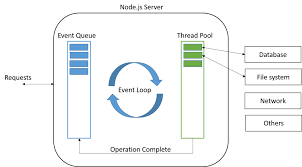
\includegraphics[scale=0.9]{figures/js-event-loop.png}
	\centering
	\caption{Βρόχος συμβάντων της \selectlanguage{english}\textit{JavaScript}\selectlanguage{greek} (Πηγή: \cite{[JS3]})}
	\label{eventloop}
\end{figure}

\subsubsection{\selectlanguage{english}Run to Completion Logic\selectlanguage{greek}}

Η πρακτική που ακολουθεί το περιβάλλον της \selectlanguage{english}JavaScript\selectlanguage{greek} είναι η πλήρης
επεξεργασία κάθε μηνύματος προτού συνεχίσει με το επόμενο. Αυτό προσφέρει
κάποιες ελκυστικές ιδιότητες κατά το σχεδιασμό της λογικής των προγραμμάτων, συμπεριλαμβανομένης της εγγύησης της εγκυρότητας των δεδομένων κατά τη διάρκεια της εκτέλεσης συναρτήσεων. Παρατηρείται δηλαδή διαφορά με το μοντέλο της \selectlanguage{english}C\selectlanguage{greek}, κατά το οποίο, όταν μία συνάρτηση ή κομμάτι κώδικα εκτελείται μέσα σε κάποιο νήμα, το σύστημα έχει τη δυνατότητα να διακόψει την εκτέλεσή τους και να μεταφέρει τον έλεγχο σε κάποιο άλλο νήμα. Βέβαια, υπάρχουν και μειονεκτήματα στην προσέγγιση αυτή, το σπουδαιότερο εκ των οποίων έχει να κάνει με το εάν ένα μήνυμα χρειαστεί σημαντικό χρονικό διάστημα για την επεξεργασία του, όλη η εφαρμογή καθίσταται ανίκανη να διαχειριστεί οποιαδήποτε αλληλεπίδραση με το χρήστη. Δεν είναι σπάνια, ακόμα και σήμερα, η εμφάνιση ειδοποίησης με τη μορφή ξεχωριστού παραθύρου από τον \selectlanguage{english}browser\selectlanguage{greek}, σύμφωνα με την οποία «η εκτέλεση κάποιου \selectlanguage{english}script\selectlanguage{greek} καθιστά την εφαρμογή μη αποκρίσιμη». Οι προγραμματιστές για να υπερκεράσουν τους περιορισμούς αυτούς προσπαθούσαν να μειώσουν όσο γίνεται το χρόνο επεξεργασίας που απαιτείτο ή, αν
αυτό δεν ήταν δυνατό, να «μοιράσουν» το φόρτο σε μικρότερα μηνύματα, τα οποία τοποθετούσαν εκ νέου στο βρόχο συμβάντων χρησιμοποιώντας ειδικά \selectlanguage{english}API calls\selectlanguage{greek}, όπως \selectlanguage{english}\textit{setTimeout()}\selectlanguage{greek} και \selectlanguage{english}\textit{setInterval()}\selectlanguage{greek}.

\subsubsection{\selectlanguage{english}Asynchronous JavaScript and XML}
\selectlanguage{greek}

Όπως έχει ήδη αναφερθεί, στο παρελθόν η \selectlanguage{english}HTML\selectlanguage{greek} αποτελούσε τη μοναδική προσέγγιση στατικών ιστοσελίδων και \selectlanguage{english}web\selectlanguage{greek} υπηρεσιών. Η εμφάνιση της \selectlanguage{english}JS\selectlanguage{greek} προσσέγισης έφερε την πραγματική επανάσταση στην ανάπτυξη εφαρμογών και διαδικτυακών προγραμμάτων. Σε αυτό συνέβαλλε κυρίως η εμφάνιση των \selectlanguage{english}AJAX\selectlanguage{greek} τεχνικών \cite{[AJAX1],[AJAX2]}, οι οποίες μετατόπισαν τον έλεγχο της ροής και της πληροφορίας από τους εξυπηρετητές στους πελάτες. Ο \selectlanguage{english}client side\selectlanguage{greek} προγραμματισμός έχει αναβαθμιστεί και πλέον είναι εφικτή η αλληλεπίδραση μεταξύ του \selectlanguage{english}backend\selectlanguage{greek} και του \selectlanguage{english}frontend\selectlanguage{greek} μιας εφαρμογής μέσω αμοιβαίων ασύγχρονων αιτημάτων. Με αυτό τον τρόπο, ο \selectlanguage{english}client\selectlanguage{greek} μπορεί να αιτηθεί δεδομένα από τον \selectlanguage{english}server\selectlanguage{greek} και, όταν αυτά είναι διαθέσιμα, να τα αναπαραστήσει ή να τα επεξεργαστεί κατάλληλα.


\subsubsection{\selectlanguage{english}Single Page Applications}
\selectlanguage{greek}
Η επόμενη καθοριστική αλλαγή ήρθε το 2002 με την είσοδο της έννοιας των εφαρμογών μονής σελίδας \textit{\textbf{--}} \selectlanguage{english}\textit{SPA}\selectlanguage{greek}. H λογική εδώ είναι ότι μια \selectlanguage{english}web\selectlanguage{greek} εφαρμογή λαμβάνει χώρα σε μία μόνο ιστοσελίδα με στόχο να παρέχει μια πιο άμεση και ομαλή
εμπειρία συγκρίσιμη με εφαρμογές επιφάνειας εργασίας (\selectlanguage{english}desktop applications\selectlanguage{greek}). Η σελίδα φορτώνεται μία μόνο φορά και στη συνέχεια τα δεδομένα φορτώνονται δυναμικά μέσω αλληλεπίδρασης \selectlanguage{english}server \textit{\textbf{--}} client\selectlanguage{greek}, ενώ ταυτόχρονα εξακολουθεί να δίνει στον χρήστη την εντύπωση οτι πλοηγείται σε διαφορετικές σελίδες, εντός της εφαρμογής \cite{[SPA1]}.

\begin{figure}[ht]
	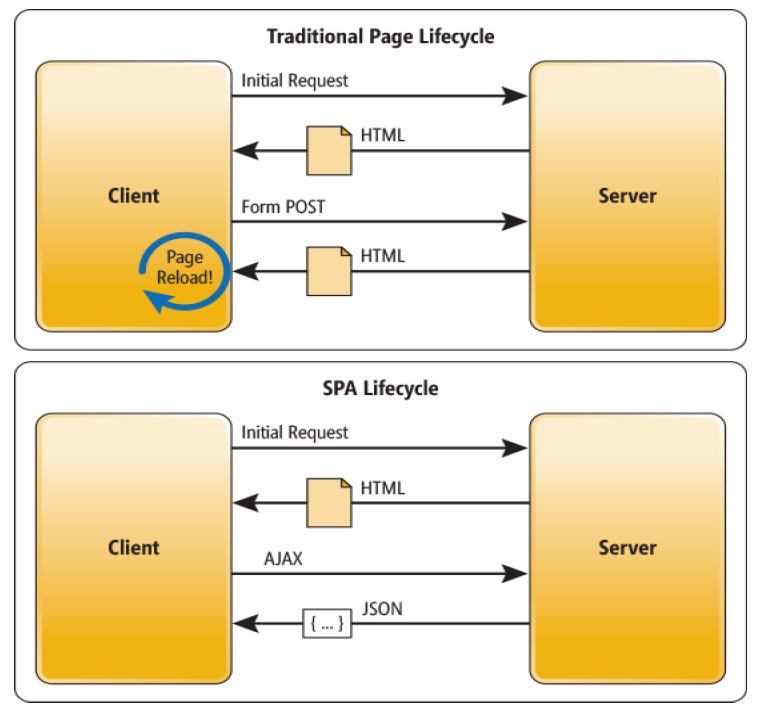
\includegraphics[scale=0.5]{figures/ajax-calls.png}
	\centering
	\caption{Διαφορές μεταξύ παραδοσιακής λογικής ιστοσελίδας και λογικής \selectlanguage{english}\textit{SPA}\selectlanguage{greek}.}
	\label{ajaxcalls}
\end{figure}

Αυτή η στροφή στον τρόπο διαχείρισης δεδομένων, κατέρριψε τα εμπόδια μεταξύ απόδοσης και πολυπλοκότητας.

\subsubsection{\selectlanguage{english}Model View Controller}
\selectlanguage{greek}
Ωστόσο, πολυπλοκότητα και η ποσότητα της λογικής που δόθηκε στον πελάτη
δημιούργησε νέα προβλήματα. Το μέγεθος του κώδικα αυξήθηκε δραματικά, και οι τεχνοτροπίες που δημιουργήθηκαν ποίκιλλαν πολύ. H λύση δόθηκε ομαδοποιώντας πρακτικές και σχεδιαστικές επιλογές σε ολοκληρωμένες τεχνοτροπίες (\selectlanguage{english}frameworks\selectlanguage{greek}) που μέχρι στιγμής υπήρχαν μόνο στους εξυπηρετητές. Η πιο γνωστή όλων
αυτών των \selectlanguage{english}JavaScript Frameworks\selectlanguage{greek} είναι η τεχνοτροπία Μοντέλου \textit{\textbf{--}} Όψης \textit{\textbf{--}} Ελεγκτή, γνωστή και ως \selectlanguage{english}\textit{MVC}\selectlanguage{greek}(βλ. Σχ. \ref{mvcmodel}), η οποία αποτελείται από τα εξής τρία μέρη:

\begin{itemize}
\item \textbf{Μοντέλα \textit{\textbf{--}} \selectlanguage{english}\textit{Models}\selectlanguage{greek}} που αναπαριστούν τις σχετικές με την εφαρμογή πληροφορίες
και δεδομένα, όπως συγκεκριμένες κλάσεις-δοχεία (\selectlanguage{english}container classes\selectlanguage{greek}) δεδομένων. Τα μοντέλα μπορούν να ενημερώνουν τυχόν παρατηρητές όταν η κατάστασή τους αλλάζει (π.χ. όταν κάποια πληροφορία που κρατούν ενημερώνεται ή διαγράφεται) \cite{[MVC1]}.
\item \textbf{Όψεις \textit{\textbf{--}} \selectlanguage{english}\textit{Views}\selectlanguage{greek}} που τυπικά θεωρούνται ως η διεπαφή του χρήστη με την εφαρμογή
(π.χ. ο κώδικας \selectlanguage{english}HTML\selectlanguage{greek} και \selectlanguage{english}CSS\selectlanguage{greek}). Πρέπει να γνωρίζουν για την ύπαρξη των
μοντέλων, έτσι ώστε να τα παρατηρούν, αλλά δεν επικοινωνούν κατευθείαν μαζί
τους.
\item \textbf{Ελεγκτές \textit{\textbf{--}} \selectlanguage{english}\textit{Controllers}\selectlanguage{greek}} που υλοποιούν τη λογική παρουσίασης (\selectlanguage{english}presentation logic\selectlanguage{greek})
της εφαρμογής. Αυτοί είναι που παίρνουν τις αποφάσεις και ο συνδετικός κρίκος μεταξύ Μοντέλων και Όψεων.
\end{itemize}

\begin{figure}[ht]
	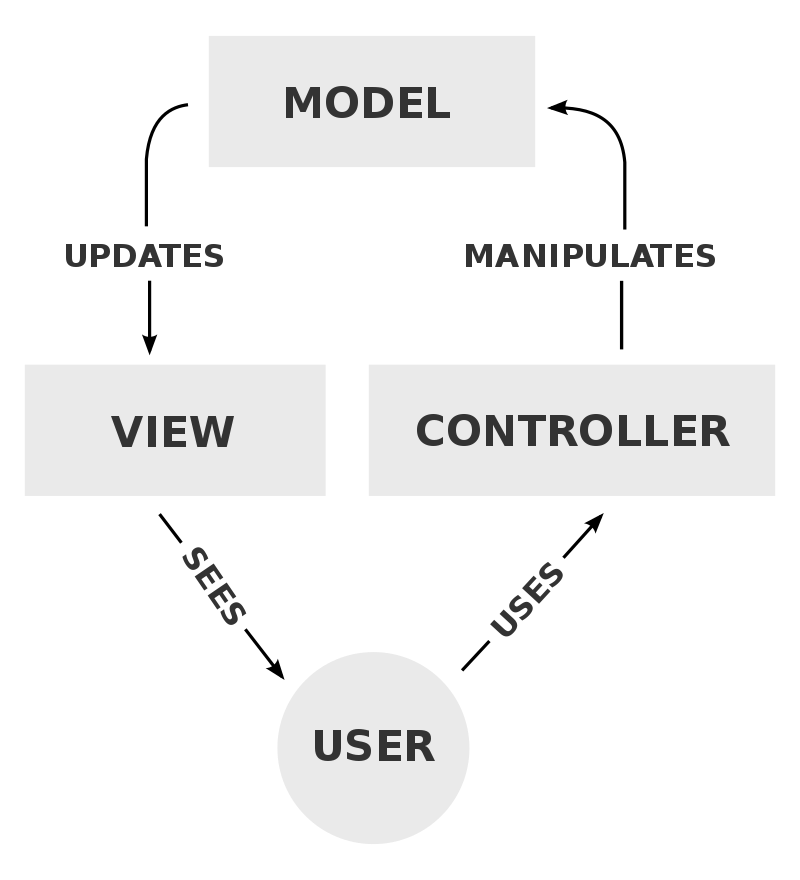
\includegraphics[scale=0.2]{figures/mvc-model.png}
	\centering
	\caption{Διάγραμμα αναπαράστασης των αλληλεπιδράσεων βάσει του μοντέλου \selectlanguage{english}\textit{MVC}\selectlanguage{greek}.}
	\label{mvcmodel}
\end{figure}


\subsection{Η Ανάγκη Μιας Νέας Τεχνολογίας - \selectlanguage{english}React Framework}
\selectlanguage{greek}
Ωστόσο, η αύξηση της πολυπλοκότητας των \selectlanguage{english}mobile applications\selectlanguage{greek} συνεπάγεται αύξηση των απαιτήσεων. Πλέον, η ανάπτυξη μιας \selectlanguage{english}native\selectlanguage{greek} εφαρμογής συνοδεύεται από πολλαπλά καθήκοντα. H υλοποίηση κώδικα που μπορεί να μεταφερθεί με ελάχιστες τροποποιήσεις μεταξύ πολλαπλών πλατφόρμων (\selectlanguage{english}cross-platform apps\selectlanguage{greek}), η ανάγκη για εφαρμογές που υποστηρίζονται και από το \selectlanguage{english}web (web apps)\selectlanguage{greek}, το συνολικό κόστος ανάπτυξης, καθώς και ο χρόνος ανάπτυξης είναι μερικοί από τους βασικότερους παράγοντες που συνέδραμαν στην αναζήτηση μιας καινοτόμου λύσης.

Έτσι, το 2011 η ομάδα προγραμματιστών του \selectlanguage{english}Facebook\selectlanguage{greek} διαμόρφωσε μια νέα τεχνολογία για την ανάπτυξη \selectlanguage{english}web\selectlanguage{greek} και \selectlanguage{english}native\selectlanguage{greek} εφαρμογών, γνωστή ως \selectlanguage{english}React\selectlanguage{greek} (\selectlanguage{english}\textit{React.js}\selectlanguage{greek} ή \selectlanguage{english}\textit{ReactJS}\selectlanguage{greek}). Τα βασικότερα χαρακτηριστικά της\selectlanguage{english} React\selectlanguage{greek} είναι:

\begin{itemize}
\item η αρχιτεκτονική διαίρεσης του κώδικα σε μικρότερα στοιχεία, τα οποία καλούνται \selectlanguage{english}components (component-based architecture)\selectlanguage{greek} \cite{[REACT1]},
\item η μονοσήμαντη ροή δεδομένων μέσω των ``\textit{ιδιοτήτων}'' (\selectlanguage{english}\textit{props}\selectlanguage{greek}) ενός στοιχείου (\selectlanguage{english}one-way data binding\selectlanguage{greek}) \cite{[REACT1]},
\item η δυνατότητα αποθήκευσης της κατάστασης ενός στοιχείου (\selectlanguage{english}stateful component\selectlanguage{greek}) και μετάδοσης της κατάστασης (\selectlanguage{english}state\selectlanguage{greek}) σε στοιχεία-παιδιά (\selectlanguage{english}child-component\selectlanguage{greek}) του στοιχείου-πατέρα (\selectlanguage{english}parent-component\selectlanguage{greek}) μέσω των \selectlanguage{english}props\selectlanguage{greek},
\item η \selectlanguage{english}JSX\selectlanguage{greek} σύνταξη \cite{[REACT3]}
\item η ανανέωση μόνο εκείνου του περιεχομένου της σελίδας που μεταββάλεται (\selectlanguage{english}virtual DOM\selectlanguage{greek}) \cite{[REACT2]} και
\item η δυνατότητα εκτέλεσης τμημάτων κώδικα σε δεδομένα χρονικά σημεία κατά τον κύκλο ζωής του στοιχείου με τη βοήθεια συγκεκριμένων \selectlanguage{english}hooks\selectlanguage{greek} (\selectlanguage{english}lifecycle methods\selectlanguage{greek}), τα βασικότερα εκ των οποίων είναι \textit{\selectlanguage{english}render(), componentDidMount(), componentWillUnmount()\selectlanguage{greek}}
\end{itemize}

H φιλοσοφία ενιαίου κώδικα σε όλες τις πλατφόρμες απέκτησε δημοτικότητα με ραγδαίους ρυθμούς. Ως αποτέλεσμα, η κοινότητα προγραμματιστών του \selectlanguage{english}Facebook\selectlanguage{greek} σηματοδότησε επισήμως το 2015 την έναρξη μιας νέας εποχής, με την ανακοίνωση της \selectlanguage{english}React Native\selectlanguage{greek}. 
 
\selectlanguage{english}
\begin{lstlisting}[language=React, caption=\selectlanguage{greek}Παράδειγμα κώδικα σε \selectlanguage{english}React\selectlanguage{greek} (Πηγή:\cite{[REACT4]})]
class Board extends React.Component {
  constructor(props) {
    super(props);
    this.state = {
      squares: Array(6).fill(null),
    };
  }

  handleClick(i) {
    const squares = this.state.squares.slice();
    squares[i] = 'X';
    this.setState({squares: squares});
  }

  renderSquare(i) {
    return (
      <Square
        value={this.state.squares[i]}
        onClick={() => this.handleClick(i)}
      />
    );
  }

  render() {
    const status = 'Next player: X';
    return (
      <div>
        <div className="status">{status}</div>
        <div className="board-row">
          {this.renderSquare(0)}
          {this.renderSquare(1)}
          {this.renderSquare(2)}
        </div>
        <div className="board-row">
          {this.renderSquare(3)}
          {this.renderSquare(4)}
          {this.renderSquare(5)}
        </div>
      </div>
    );
  }
}
\end{lstlisting}
\selectlanguage{greek}

\subsubsection{\selectlanguage{english}React Native}
\selectlanguage{greek}

Η \selectlanguage{english}React Native\selectlanguage{greek}, είναι ένα \selectlanguage{english}Framework\selectlanguage{greek} για την ανάπτυξη πραγματικών, native εφαρμογών για \selectlanguage{english}iOS\selectlanguage{greek} και \selectlanguage{english}Android\selectlanguage{greek} πλατφόρμες. Η φιλοσοφία της \selectlanguage{english}React Native\selectlanguage{greek} είναι πανονομοιότυπη με αυτή της \selectlanguage{english}React\selectlanguage{greek}, και στηρίζεται στους ίδιους κανόνες και τεχνικές που διέπουν τα πλαίσια της \selectlanguage{english}JavaScript\selectlanguage{greek}, με τη μόνη διαφορά ότι αποσκοπεί στην σχεδίαση διεπιφανειών που απευθύνονται σε πλατφόρμες κινητών συσκευών, έναντι προγραμμάτων περιήγησης. Με άλλα λόγια, αποτελεί έναν νέο τρόπο υλοποίησης εφαρμογών που δε διαφέρουν σε τίποτα από εφαρμογές γραμμένες σε \selectlanguage{english}native\selectlanguage{greek} γλώσσες προγραμματισμού (\selectlanguage{english}Swift, Java\selectlanguage{greek}). Έτσι, είναι πλέον εφικτή η ανάπτυξη εφαρμογών για πολλαπλές πλατφόρμες, με τη χρήση μιας μόνο γλώσσας, η οποία υποστηρίζεται και από τις εφαρμογές \selectlanguage{english}web\selectlanguage{greek}. Το χρονοδιάγραμμα υλοποίησης μειώνεται αισθητά, αφού η διαδικασία ανάπτυξης \selectlanguage{english}iOS\selectlanguage{greek} και \selectlanguage{english}Android\selectlanguage{greek} εφαρμογών μπορεί να γίνει τώρα παράλληλα. Εντούτοις, το κόστος ανάπτυξης της εφαρμογής δεν εξαρτάται πλέον από τη δυνατότητα ή μη υποστήριξης της εφαρμογής από περισσότερες από μια πλατφόρμες. 

Τα πλεονεκτήματα που προάγουν τη \selectlanguage{english}React Native\selectlanguage{greek} ως το δημοφιλέστερο \selectlanguage{english}cross-platform framework\selectlanguage{greek} είναι πολλά. Όπως και η \selectlanguage{english}React\selectlanguage{greek}, έτσι και η \selectlanguage{english}React Native\selectlanguage{greek} χρησιμοποιεί \selectlanguage{english}JSX\selectlanguage{greek} σύνταξη. Ωστόσο, στην υλοποίηση χρησιμοποιούνται οι μητρικές διεπαφές κάθε πλατφόρμας (\selectlanguage{english}Objective-C\selectlanguage{greek} για \selectlanguage{english}iOS\selectlanguage{greek} και \selectlanguage{english}Java\selectlanguage{greek} για \selectlanguage{english}Android\selectlanguage{greek}). Το γεγονός αυτό καθιστά τις εφαρμογές εξίσου αποδοτικές, με αυτές σε \selectlanguage{english}native\selectlanguage{greek} κώδικα. Έτσι, οι προγραμματιστές που είναι εξοικειωμένοι με την ανάπτυξη \selectlanguage{english}web\selectlanguage{greek} εφαρμογών μπορούν να εκμεταλλευτούν τη συγγένεια των δύο αυτών γλωσσών.

\paragraph{Προγραμματιστική Εμπειρία \textbf{--} \selectlanguage{english}Developer Experience\selectlanguage{greek}} 
\paragraph{}
Για προγραμματιστές με προϋπάρχουσα εμπειρία στην ανάπτυξη \selectlanguage{english}mobile\selectlanguage{greek} εφαρμογών, το περιβάλλον της \selectlanguage{english}React Native\selectlanguage{greek} είναι ιδιαίτερα φιλικό. Η ομάδα της \selectlanguage{english}React Native\selectlanguage{greek} προσφέρει στον προγραμματιστή ισχυρά προγραμματιστικά εργαλεία που διευκολύνουν τη διαδικασία ανάπτυξης μιας εφαρμογής και μειώνουν αισθητά το χρόνο προγραμματισμού. Για παράδειγμα, δεν απαιτείται \selectlanguage{english}rebuild\selectlanguage{greek} κάθε φορά που ο προγραμματιστής επιθυμεί να προβάλλει τις αλλαγές στην εφαρμογή, αλλά αρκεί μια απλή ανανέωση της σελίδας, όπως σε μια συνηθισμένη ιστοσελίδα. Αυτό εντίνει ιδιαίτερα την αμεσότητα στη διαδικασία επικοινωνίας μεταξύ κώδικα και εφαρμογής και έτσι ο προγραμματιστής μπορεί να ελέγχει τις αλλαγές του κάθε φορά. Αυτό έχει σημαντικό αντίκτυπο στην περίπτωση σχεδιασμού (\selectlanguage{english}design\selectlanguage{greek}) της εφαρμογής, όπου λεπτομερείς αλλαγές λαμβάνουν χώρα διαρκώς και η εφαρμογή μπορεί να ανανεώνεται αυτομάτως.    

Επίσης, το περιβάλλον υποστήριξης της \selectlanguage{english}React Native\selectlanguage{greek} συνοδεύεται από ολοκληρωμένη και επικαιροποιημένη βιβλιογραφία, ενώ σημαντική προσοχή δίνεται και στη διαδικασία αποσφαλμάτωσης του κώδικα μέσω επεξηγηματικών μηνυμάτων λάθους. Ο προγραμματιστής μπορεί να επωφεληθεί από τα έξυπνα εργαλεία εντοπισμού σφαλμάτων και την αναφορά σφαλμάτων που είναι ενσωματωμένα στους σύγχρονους περιηγητές όπως ο \selectlanguage{english}Chrome\selectlanguage{greek} ή ο \selectlanguage{english}Safari\selectlanguage{greek} (βλ. Σχ. \ref{debugger}). Παρομοίως, η ίδια ευελιξία χαρακτηρίζει και την επιλογή της πλατφόρμας προγραμματισμού, καθώς ο προγραμματιστής είναι ελεύθερος να επιλέξει εκείνο τον \selectlanguage{english}text editor\selectlanguage{greek} με τον οποίο διαθέτει τη μέγιστη εξοικείωση. Περιορισμοί όπως ο προγραμματισμός σε συγκεκριμένο λογισμικό για εφαρμογές \selectlanguage{english}iOS\selectlanguage{greek} ή \selectlanguage{english}Android\selectlanguage{greek}, που χαρακτηρίζουν τις \selectlanguage{english}native\selectlanguage{greek} γλώσσες προγραμματισμού (όπως αναφέρθηκε στην ενότητα 2.3.2) δεν αποτελούν εμπόδιο για την \selectlanguage{english}React Native\selectlanguage{greek}. Όλα τα παραπάνω συνεισφέρουν σε μία πρωτοποριακή και εποικοδομητική εμπειρία, που επιτρέπει την επικέτρωση στο προγραμματιστικό κομμάτι και εξασφαλίζει ταχύτητα και ευκολία.

\begin{figure}
    \centering
    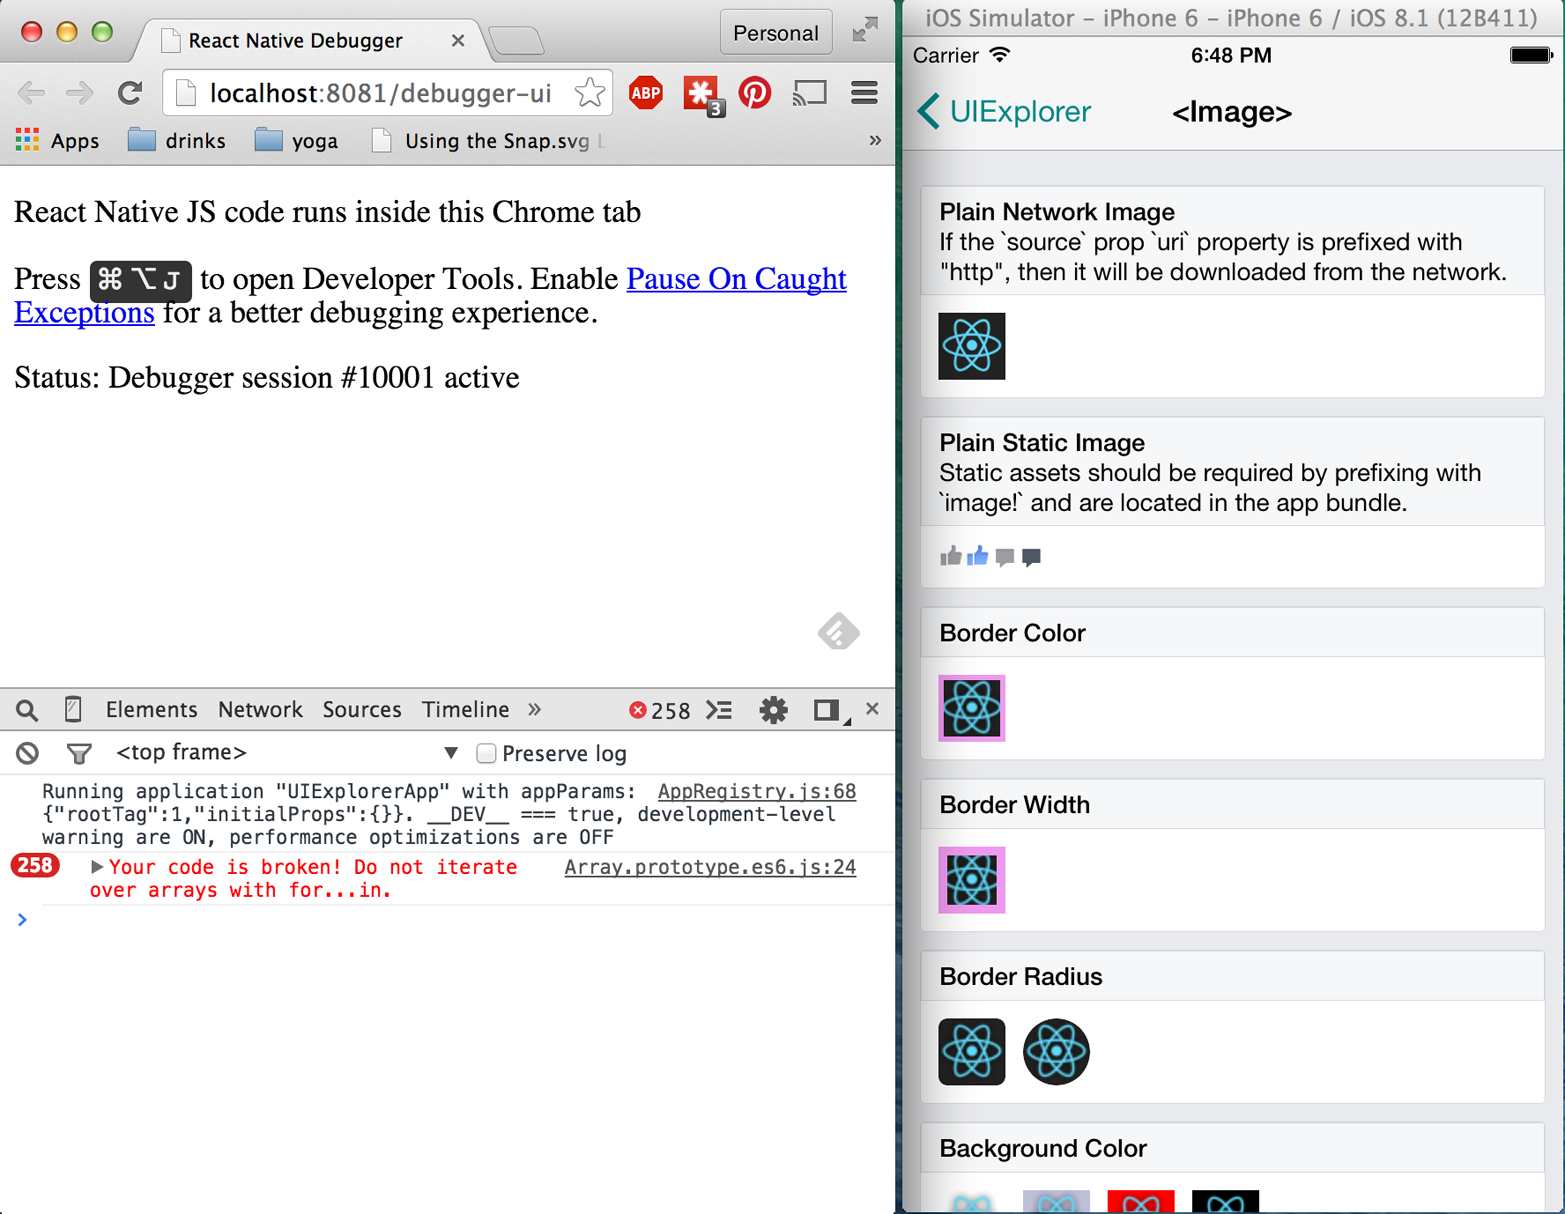
\includegraphics[scale=0.9]{figures/using-react-native-debugger.png}
    \caption{Χρήση του ενσωματωμένου αποσφαλματωτή στον περιηγητή \selectlanguage{english}Chrome\selectlanguage{greek}}
    \label{debugger}
\end{figure}

\paragraph{Επαναχρησιμότητα και Κοινή Χρήση \textbf{--} \selectlanguage{english}Code Reuse and Knowlegde Sharing\selectlanguage{greek}} 
\paragraph{}

Η εργασία στο περιβάλλον της \selectlanguage{english}React Native\selectlanguage{greek} μπορεί να ελαχιστοποιήσει δραματικά τους απαιτούμενους πόρους για την ανάπτυξη μιας \selectlanguage{english}mobile\selectlanguage{greek} εφαρμογής. Οποιοσδήποτε διαθέτει γνώση της \selectlanguage{english}React\selectlanguage{greek} μπορεί να στοχεύσει την ανάπτυξη, τόσο \selectlanguage{english}web\selectlanguage{greek} εφαρμογών, όσο και \selectlanguage{english}native\selectlanguage{greek} (\selectlanguage{english}iOS\selectlanguage{greek} και \selectlanguage{english}Android\selectlanguage{greek}) χωρίς περιορισμούς. Έτσι, παύει να υπάρχει διάκριση μεταξύ προγραμματιστών. Χρησιμοποιώντας το ίδιο σύνολο δεξιοτήτων και γνώσεων, κάθε ομάδα προγραμματιστών μπορεί να εργαστεί ταχύτερα, αμεσότερα και αποτελεσματικότερα, αφού η γνώση είναι κοινή και μπορεί να μοιραστεί ανά πάσα στιγμή.

Εκτός από την κοινή χρήση της γνώσης, μεγάλα τμήματα κώδικα μπορούν επίσης να επαχρησιμοποιηθούν. Προφανώς, ενδέχετεαι η απαίτηση περαιτέρω τροποποίησης κάποιων σημείων του κώδικα που αφορά κάθε πλατφόρμα. Παρ' όλα αυτά, η επαναχρησιμοποίηση κώδικα μεταξύ διαφόρων πλατφόρμων είναι ιδιαίτερα εύκολη και γρήγορη. Αρκούν κάποιες συνθήκες και η χρήση κάποιων διαφορετικών διεπαφών προκειμένου να καταστεί εφικτή η \selectlanguage{english}cross-platform\selectlanguage{greek} λειτουργικότητα. Για παράδειγμα, η εφαρμογή διαχείρισης διαφημίσεων του \selectlanguage{english}Facebook\selectlanguage{greek} για \selectlanguage{english}Android\selectlanguage{greek} μοιράζεται το 87\% της βάσης του κώδικα με την αντίστοιχη εφαρμογή για \selectlanguage{english}iOS\selectlanguage{greek} \cite{[RN1]}.

\paragraph{Εξοικονόμηση Πόρων \textbf{--} \selectlanguage{english}Resource Saving\selectlanguage{greek}} 
\paragraph{}

Στην εποχή αυτή της τεχνολογίας, συναντάται συχνά η απαίτηση υψηλής ποιότητας με χαμηλό κόστος. Η \selectlanguage{english}React Native\selectlanguage{greek} θεμελιώνεται σε αυτά τα δεδομένα, προσφέροντας υψηλή απόδοση με ελαχιστοποίηση των απαιτούμενων πόρων. Οι περισσότερες ηλεκτρονικές υπηρεσίες και εταιρείες σήμερα έχουν την ανάγκη να αντιπροσωπεύονται τόσο στο διαδίκτυο μέσω μιας \selectlanguage{english}web\selectlanguage{greek} εφαρμογής, όσο και στις φορητές συσκευές μέσω \selectlanguage{english}native\selectlanguage{greek} εφαρμογών. Το γεγονός ότι η χρήση φορητών συσκευών αυξάνεται με εκθετικούς ρυθμούς την τελευταίες δεκαετίες (βλ. Σχ. \ref{mobileusage}), έχει στρέψει την προσοχή στην δεύτερη κατηγορία εφαρμογών.  Όπως προαναφέρθηκε, είναι πλέον εφικτή η ανάπτυξη μιας εφαρμογής που ανταποκρίνεται σε πολλές πλατφόρμες, με ελάχιστες τροποποιήσεις. Ως αποτέλεσμα, οι ομάδες προγραμματιστών εντός μιας εταιρείας είναι μικρότερες και πιο ευέλικτες. Ακόμη, τα χρονικά πλαίσια ολοκλήρωσης μιας εφαρμογής είναι συντομότερα και δεν αυξάνονται ανάλογα με τον αριθμό πλατφόρμων υποστήριξης της εφαρμογής, όπως άλλοτε. Τέλος, είναι ευνόητο πως τα παραπάνω ευνοούν την εξοικονόμηση χρηματικών πόρων που απαιτούνται για την ανάπτυξη μιας εφαρμογής \cite{[RN2]}. Αναμφισβήτητα λοιπόν, η \selectlanguage{english}React Native\selectlanguage{greek} αποκτά μεγάλη δημοτικότητα και για αυτούς τους λόγους, γνωστές εφαρμογές όπως η \selectlanguage{english}AirBnB\selectlanguage{greek}, το \selectlanguage{english}Skype\selectlanguage{greek}, το \selectlanguage{english}Instagram\selectlanguage{greek} και το \selectlanguage{english}Facebook\selectlanguage{greek} την έχουν υιοθετήσει \cite{[RN3]}.

\begin{figure}
    \centering
    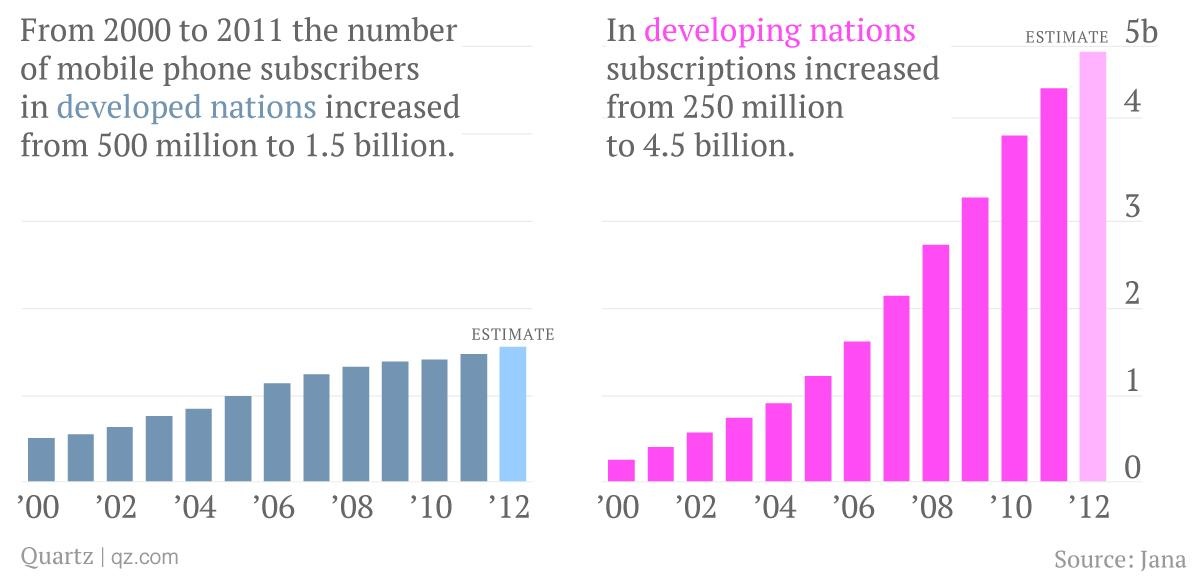
\includegraphics[scale=0.4]{figures/mobile-use.png}
    \caption{Η χρήση εφαρμογών σε κινητά αυξάνεται εκθετικά.}
    \label{mobileusage}
\end{figure}


\subsubsection{\selectlanguage{english}React Native Bridge}
\selectlanguage{greek}

Η φιλοσοφία πίσω από τον τρόπο λειτουργίας της \selectlanguage{english}React Native\selectlanguage{greek} είναι απλή. Προκειμένου να προσφέρει στον προγραμματιστή την ίδια εμπειρία με τις \selectlanguage{english}native\selectlanguage{greek} εφαρμογές, χρησιμοποιεί πανομοιότυπες διεπαφές και διεπιφάνειες με τις αντίστοιχες των \selectlanguage{english}native\selectlanguage{greek} γλωσσών. Πιο συγκεκριμένα, η \selectlanguage{english}React Native\selectlanguage{greek} απαρτίζεται από δύο τμήματα (\selectlanguage{english}realms\selectlanguage{greek}): 

\begin{itemize}
    \item το τμήμα της \selectlanguage{english}JavaScript (JavaScript Realm)\selectlanguage{greek} και
    \item το τμήμα των \selectlanguage{english}Native UIs (Native Realm)\selectlanguage{greek}
\end{itemize} 

Τα δύο τμήματα επικοινωνούν μεταξύ τους χρησιμοποιώντας μια ``\textit{γέφυρα}'' (\selectlanguage{english}bridge\selectlanguage{greek}), η οποία αποτελεί αναμφισβήτητα τον πυρήνα της αρχιτεκτονικής της \selectlanguage{english}React Native\selectlanguage{greek} (βλ. Σχ. \ref{reactnativebridge}). Η γεφύρωση αυτή των δύο παραπάνω τμηματων, αν και υλοποιημένη σε διαφορετικές τεχνολογίες, αποτελεί ουσιαστικά την βασική έννοια που προσφέρει τη δυνατότητα της αμφίδρομης και ασύγχρονης επικοινωνίας αυτών \cite{[RN4]}. Η επικοινωνία αυτή επιτυγχάνεται με τη χρήση διαλειτουργικών γλωσσών (\selectlanguage{english}interoperable languages\selectlanguage{greek}) όπως \selectlanguage{english}XML, JSON\selectlanguage{greek} κλπ. Περισσότερα για αυτές θα δούμε σε παρακάτω ενότητα (βλ. ενότητα 2.4.3).

\begin{figure}
    \centering
    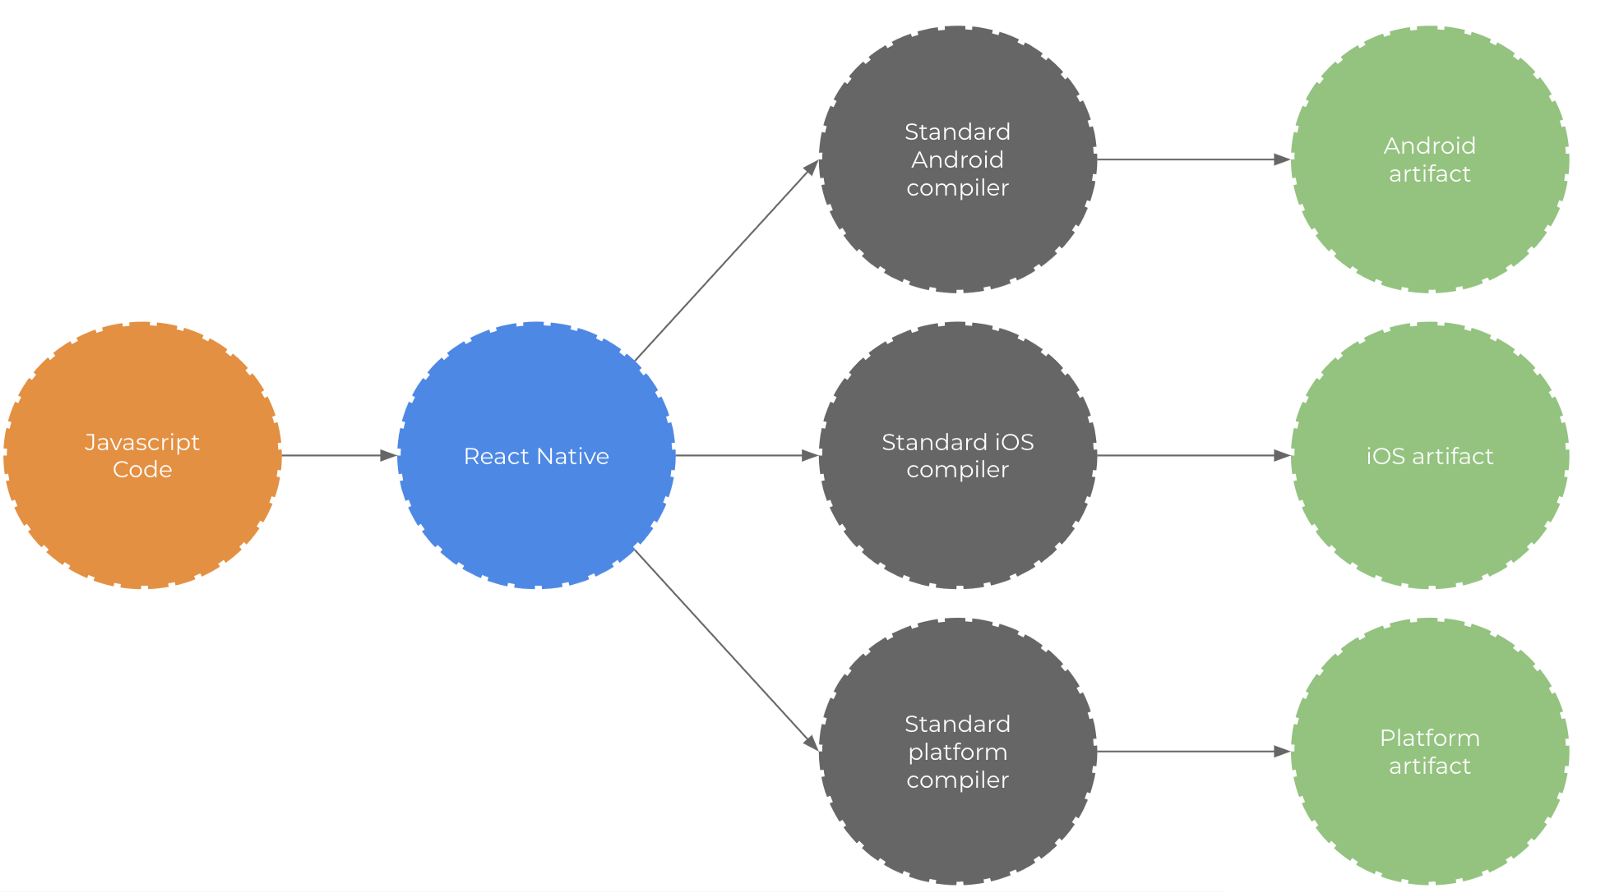
\includegraphics[scale=0.2]{figures/react-native-bridge.png}
    \caption{Η \selectlanguage{english}React Native\selectlanguage{greek} χρησιμοποιεί τα ίδια \selectlanguage{english}native UIs\selectlanguage{greek}, όπως η \selectlanguage{english}Java\selectlanguage{greek} για \selectlanguage{english}Andorid\selectlanguage{greek} και η \selectlanguage{english}Swift\selectlanguage{greek} για \selectlanguage{english}iOS\selectlanguage{greek}}
    \label{reactnativebridge}
\end{figure}

\section{Πρόσθετες Τεχνολογικές Έννοιες}
\subsection{\selectlanguage{english}Node.js}
\selectlanguage{greek}

Το \selectlanguage{english}Node.js\selectlanguage{greek} (συχνά αναφερόμενο και ως \selectlanguage{english}Node\selectlanguage{greek}) είναι ένα περιβάλλον ανοικτού κώδικα με την υποστήριξη από πολλές πλατφόρμες. Το μεγαλύτερο μέρος του είναι γραμμένο στη γλώσσα \selectlanguage{english}Javascript\selectlanguage{greek}. Το \selectlanguage{english}Node.js\selectlanguage{greek} χρησιμοποιεί τεχνικές εισόδου/εξόδου χωρίς αποκλεισμό (\selectlanguage{english}non-blocking I/O\selectlanguage{greek}), με αποτέλεσμα να παραμένει εύχρηστο και ελαφρύ όταν έρχεται αντιμέτωπο με εφαρμογές έντονου φορτίου πραγματικού χρόνου, με υψηλές απαιτήσεις μεταφοράς δεδομένων \cite{[NODE1]}. Το \selectlanguage{english}non-blocking\selectlanguage{greek} μέρος σημαίνει ότι κάποιες εντολές, όπως ανάγνωση από αρχείο, μεταβιβάζονται και εκτελούνται παράλληλα και χρησιμοποιούν μεθόδους ανάκλησης (\selectlanguage{english}callback functions\selectlanguage{greek}) για να ολοκληρώσουν το μήνυμα. Σε μία γλώσσα όπως η \selectlanguage{english}\textit{PHP}\selectlanguage{greek} για παράδειγμα, μία νέα εντολή εκτελείται μόνο αφού ολοκληρωθεί η εκτέλεση της προηγούμενης εντολής \cite{[NODE2]}. Η τεχνολογία \selectlanguage{english}Node\selectlanguage{greek} δεν είναι σχεδιασμένη να παρέχει σύνθετη υπολογιστική ισχύ σε πολύπλοκα συστήματα, δεδομένου ότι αυτό θα αναιρούσε όλα τα πλεονεκτήματά της.

Η \selectlanguage{english}Node\selectlanguage{greek} είναι μονονηματική. Συνεπώς, υπολογισμοί που καταναλώνουν πόρους μπορούν να φράξουν το νήμα και να αποτρέψουν την επεξεργασία άλλων αιτημάτων. Χρησιμοποιείται καλύτερα για τη δημιουργία γρήγορων, κλιμακούμενων δικτυακών εφαρμογών, δεδομένου ότι το μεγαλύτερο πλεονέκτημά της είναι αποτελεσμάτική διαχείριση μαζικών ταυτόχρονων συνδέσεων. Ένα άλλο τεράστιο πλεονέκτημα της \selectlanguage{english}Node.js\selectlanguage{greek} είναι η ενσωματωμένη διαχείριση πακέτων χρησιμοποιώντας το εργαλείο \selectlanguage{english}\textit{NPM}\selectlanguage{greek}. Το \selectlanguage{english}NPM\selectlanguage{greek} παρέχει στον προγραμματιστή ένα ευρύ σύνολο επαναχρησιμοποιήσιμων προγραμματιστικών εργαλείων και πακέτων, τα οποία εγκαθίστανται εύκολα και χρησιμοποιούνται κατά την ανάπτυξη εφαρμογών. Είναι ένα από τα μεγαλύτερα σύνολα βιβλιοθηκών ανοικτού κώδικα, με άριστη υποστήριξη και οργανωμένη βιβλιογραφία για κάθε πακέτο ανοιχτού κώδικα που διαθέτει \cite{[NODE3]}.

Ο τρόπος λειτουργίας του \selectlanguage{english}Node.js\selectlanguage{greek} επιδεικνύεται στο Σχ. \ref{nodesystem}. Η όλη δράση του \selectlanguage{english}Node.js\selectlanguage{greek} συγκεντρώνεται στον βρόχο συμβάντων (βλ. ενότητα 2.3.3.1). Η αποστολή ενός αιτήματος μέσα στην εφαρμογή πυροδοτεί την έναρξη ενός συμβάντος, το οποίο τοποθετείται στην ουρά συμβάντων (\selectlanguage{english}event queue\selectlanguage{greek}). Ο βρόχος συμβάντων λαμβάνει το συμβάν και το επεξεργάζεται. Σε περίπτωση που είναι αδύνατη η ολοκλήρωση ενός συμβάτνος (π.χ. ανάγνωση εικόνων), τότε η επεξεργασία του ανατίθεται σε ένα από τα νήματα εργασίας (\selectlanguage{english}worker threads\selectlanguage{greek}) από τη ``\textit{δεξαμενή νημάτων-εργαζομένων}'' (\selectlanguage{english}worker thread pool\selectlanguage{greek}). Όταν ένα νήμα εργασάις ολοκληρώση την επεξεργασία ενός συμβάτνος, επιστρέφει το μήνυμα απόκρισης χρησιμοποιώντας μια μέθοδο ανάκλησης η οποία διαβιβάστηκε σε αυτήν μέσω του συμβάντος. Το αποτέλεσμα μεταβιβάζεται στην εφαρμογή μέσω μιας μορφής \selectlanguage{english}Node\selectlanguage{greek} δεσμεύσεων \cite{[NODE2]}. 

\begin{figure}[ht]
    \centering
    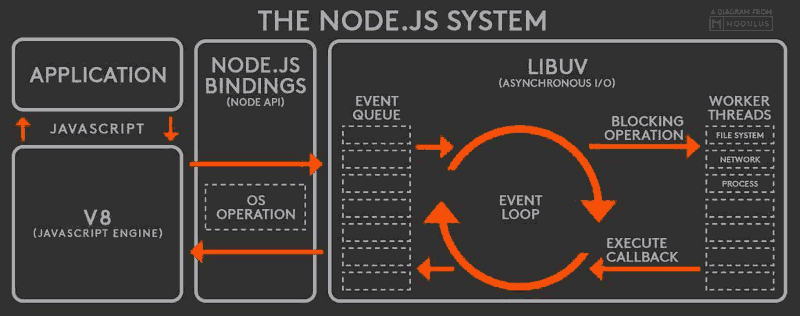
\includegraphics[scale=0.4]{figures/node-system.png}
    \caption{H αρχή λειτουργίας του συστήματος \selectlanguage{english}Node.js\selectlanguage{greek} (Πηγή: \cite{[NODE4]})}
    \label{nodesystem}
\end{figure}


Στη συνέχεια παρατίθενται τα κύρια πλεονεκτήματα της λειτουργίας ενός εξυπηρετητή \selectlanguage{english}Node.js\selectlanguage{greek}:

\begin{itemize}
    \item Ο \selectlanguage{english}Node.js server\selectlanguage{greek} μπορεί να επεξεργάζεται ασύγχρονα εισερχόμενα αιτήματα. Επομένως ο χρόνος απόκρισης είναι μικρότερος.
    \item Η \selectlanguage{english}Node.js\selectlanguage{greek} οδηγείται από συμβάντα (\selectlanguage{english}event-driven\selectlanguage{greek}) και χρησιμοποιεί \selectlanguage{english}non-blocking I/O\selectlanguage{greek}, μέσω μεθόδων επανάκλησης, του βρόχου συμβάντων και της ουράς συμβάντων. Το μοντέλο αυτό συνάδει με εκείνο των \selectlanguage{english}web servers\selectlanguage{greek}.
    \item Δεδομένου ότι βασίζεται στη \selectlanguage{english}JavaScript\selectlanguage{greek} είναι σε θέση να αξιοποιήσει το μηχανισμό \selectlanguage{english}V8 Javascript Engine\selectlanguage{greek}. Ο μηχανισμός \selectlanguage{english}V8 Javascript Engine\selectlanguage{greek} μεταγλωττίζει τον κώδικα από \selectlanguage{english}JS\selectlanguage{greek} σε κώδικα μηχανής που αποφέρει καλύτερες επιδόσεις σε σύγκριση με συνήθεις τεχνικές όπως η μετάφραση (\selectlanguage{english}interpreting\selectlanguage{greek}).
    \item Η \selectlanguage{english}Node.js\selectlanguage{greek} είναι κατάλληλη για εφαρμογές πραγματικού χρόνου που «τρέχουν» σε πολλές συσκευές. Είναι ιδανικό για γρήγορη παράδοση δεδομένων σε πολλούς αιτούντες ταυτοχρόνως.
\end{itemize}

Στο Σχ. \ref{nodevstraditional} γίνεται μια σύγκριση όσον αφορά στην επεξεργασία ενός αιτήματος μεταξύ ενός \selectlanguage{english}node server\selectlanguage{greek} και ενός συνηθισμένου \selectlanguage{english}web server\selectlanguage{greek} (όπως ο \selectlanguage{english}Apache web server\selectlanguage{greek}). Στην περίπτωση ενός \selectlanguage{english}web server\selectlanguage{greek}, σε κάθε αίτημα αντιστοιχίζεται μια νηματική διεργασία από μια δεξαμενή περιοσμένου αριθμού νημάτων. Συνεπώς, αν δεν υπάρχει διαθεσιμότητα το αίτημα τίθεται σε αναμονή έως ότου ολοκληρωθεί κάποια από τις υπόλοιπες διεργασίες. 
Η χρήση πολυνηματικών διεργασιών καταλαμβάνει αρκετό ποσοστό μνήμης στη \selectlanguage{english}RAM\selectlanguage{greek} με αποτέλεσμα την επιβράδυνση του συστήματος και άλλοτε ακόμη και τον απότομο τερματισμό αυτού. Η συμπεριφορά αυτή δεν είναι επιθυμητή. Για το λόγο αυτό, η \selectlanguage{english}Node.js\selectlanguage{greek} λειτουργεί με ένα μόνο νήμα χρησιμοποιώντας \selectlanguage{english}non-blocking I/O\selectlanguage{greek} κλήσεις, οι οποίες επιτρέπουν στο σύστημα την υποστήριξη πολλών ταυτόχρονων συνδέσεων.Για να γίνει αντιληπτό, ας υποθέσουμε ότι ο \selectlanguage{english}server\selectlanguage{greek} έχει στη διάθεσή του μια μνήμη \selectlanguage{english}RAM\selectlanguage{greek} χωρητικότητας \selectlanguage{english}8GB\selectlanguage{greek}. Επίσης, έστω ότι κάθε διεργασία καταλαμβάνει 2MB της μνήμης. Αυτό σημαίνει πως ένας παραδοσιακός web server μπορεί να επεξεργαστεί περίπου 4000 ταυτόχρονα αιτήματα. Από την άλλη πλευρά, ένας \selectlanguage{english}Node server\selectlanguage{greek} δυνητικά θα μπορούσε να επεξεργαστεί 1M ταυτόχρονα αιτήματα, χάρις την ιδιότητα επεκτασιμότητάς του \cite{[NODE1]}.

\begin{figure}[ht]
    \centering
    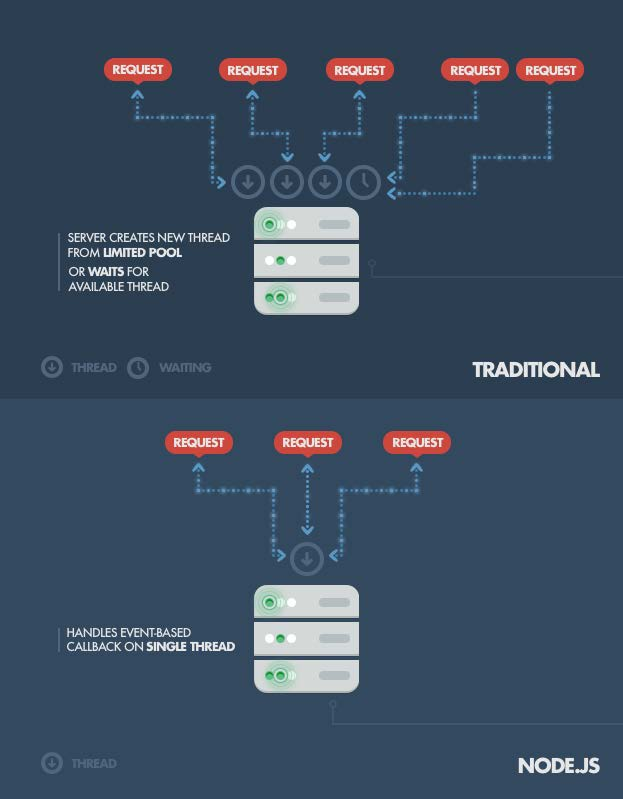
\includegraphics[scale=0.8]{figures/node-vs-tradinional-web-server.png}
    \caption{Σύγκριση ανάμεσα σε έναν \selectlanguage{english}Node.js\selectlanguage{greek} και έναν κλασσικό \selectlanguage{english}server\selectlanguage{greek}}
    \label{nodevstraditional}
\end{figure}

Εκτός από τα παραπάνω πλεονεκτήματα, ένα σημαντικό χαρακτηριστικό που καθιστά την \selectlanguage{english}Node.js\selectlanguage{greek} μία από τις κορυφαίες σύγχρονες τεχνολογίες είναι η υλοποίησή της σε \selectlanguage{english}JavaScript\selectlanguage{greek}. Το γεγονός αυτό συνεισφέρει τα μέγιστα στην ευκολία εκμάθησής της από τους προγραμματιστές που είναι ήδη εξοικειωμένοι με τη χρήση της \selectlanguage{english}JS\selectlanguage{greek}. Η προϋπόθεση της κοινής γλώσσας παίζει μείζονα ρόλο στην ανάπτυξη ολοκληρωμένων εφαρμογών (\selectlanguage{english}full stack development\selectlanguage{greek}). Έτσι, ένας προγραμματιστής έχει τη δυνατότητα να υλοποιήσει τον \selectlanguage{english}client\selectlanguage{greek} αλλά και τον \selectlanguage{english}server\selectlanguage{greek} σε μία γλώσσα (πράγμα που παλιότερα δεν ίσχυε).

\subsection{\selectlanguage{english}Representational State Transfer - REST APIs}
\selectlanguage{greek}

To \selectlanguage{english}REST\selectlanguage{greek} είναι μια μορφή αρχιτεκτονικής για τη δημιουργία δικτυακών εφαρμογών που εισήχθη το 2000 απο τον \selectlanguage{english}Roy Fielding\selectlanguage{greek} \cite{[REST2]}. Δημιουργήθηκε για να υποστηρίξει τη διαλειτουργικότητα μεταξύ όλων των υπολογιστών του διαδικτύου. Ένας \selectlanguage{english}REST Server\selectlanguage{greek} επιτρέπει την πρόσβαση πόρων μέσω κάποιου αναγνωριστικού (πχ. \selectlanguage{english}URL\selectlanguage{greek}) και ο \selectlanguage{english}REST Client\selectlanguage{greek} απλώς λαμβάνει και τροποποιεί τα δεδομένα αυτά. Οι πόροι αυτοί αναπαρίστανται με διάφορες μορφές εκ των οποίων οι πιο διαδεδομένες είναι το κείμενο, \selectlanguage{english}JSON objects, XML\selectlanguage{greek} \cite{[REST1]}. 

Η \selectlanguage{english}client\textbf{--}server\selectlanguage{greek} επικοινωνία επιτυγχάνεται μέσω αιτημάτων με ροή από τον \selectlanguage{english}client\selectlanguage{greek} στον \selectlanguage{english}server\selectlanguage{greek}. Tα αιτήματα αυτά εκκινούν από τον \selectlanguage{english}client\selectlanguage{greek} με ένα αναγνωριστικό (πχ. \selectlanguage{english}URL\selectlanguage{greek}) που αναδεικνύει τη φύση του αιτήματος, το οποίο συμβαδίζει με το endpoint που έχει δημιουργηθεί από την πλευρά του \selectlanguage{english}server\selectlanguage{greek}. Ο \selectlanguage{english}server\selectlanguage{greek} διαθέτει δρομολογητές (\selectlanguage{english}routers\selectlanguage{greek}) που αντιστοιχούν σε κάθε \selectlanguage{english}endpoint\selectlanguage{greek}. Κάθε \selectlanguage{english}router\selectlanguage{greek} έχει συγκεκριμένο ρόλο που εξυπηρετεί το αίτημα του \selectlanguage{english}client\selectlanguage{greek}. Τέλος, ο \selectlanguage{english}server\selectlanguage{greek} επιστρέφει το φορτίο (\selectlanguage{english}response payload\selectlanguage{greek}) που περιέχει τα ζητούμενα δεδομένα στον \selectlanguage{english}client\selectlanguage{greek}. Οι διεπαφές που βασίζονται σε αυτή την τεχνική ονομάζονται \selectlanguage{english}RESTful API\selectlanguage{greek} \cite{[REST3]}. Οι βασικότερες από τις διαθέσιμες μέθοδους με τις οποίες μπορεί να επιτευχθεί η παραπάνω διαδικασία είναι οι εξής:

\begin{itemize}
    \item \selectlanguage{english}\textbf{\textit{GET} --}\selectlanguage{greek}  λήψη δεδομένων από ένα \selectlanguage{english}endpoint\selectlanguage{greek}
    \item \selectlanguage{english}\textbf{\textit{POST} --}\selectlanguage{greek} αποστολή δεδομένων για αποθήκευση στο προοριζόμενο \selectlanguage{english}endpoint\selectlanguage{greek}
    \item \selectlanguage{english}\textbf{\textit{PUT} --}\selectlanguage{greek} επεξεργασία αποθηκευμένων δεδομένων στο προοριζόμενο \selectlanguage{english}endpoint\selectlanguage{greek}
     \item \selectlanguage{english}\textbf{\textit{DELETE} --}\selectlanguage{greek} διαγραφή δεδομένων από το προοριζόμενο \selectlanguage{english}endpoint\selectlanguage{greek}
\end{itemize}

Ακολουθεί επεξηγηματικός πίνακας με τις μεθόδους και την βασική αρχή λειτουργίας τους.

\begin{table}[h]
\centering
\begin{tabular}{ |m{5cm}||m{2.3cm}|m{2.3cm}|m{2.3cm}|m{2.3cm}|  }
\hline
\multicolumn{5}{|c|}{\selectlanguage{english}HTTP Methods\selectlanguage{greek}} \\
\hline 
\textit{\textbf{\selectlanguage{english}URI\selectlanguage{greek}}} & \textit{\selectlanguage{english}\textbf{GET}\selectlanguage{greek}} & \textit{\textbf{\selectlanguage{english}POST\selectlanguage{greek}}} & \textit{\textbf{\selectlanguage{english}PUT\selectlanguage{greek}}} & \textit{\textbf{\selectlanguage{english}DELETE\selectlanguage{greek}}}  \\
\hline 
\selectlanguage{english}\small{\textbf{Collection resource example}} \scriptsize{\textit{https://api.example.com/collection/}} \selectlanguage{greek}
 & \selectlanguage{english}\textit{Retrieve} the URIs of the member resources of the collection resource in the response body.\selectlanguage{greek} & \selectlanguage{english}\textit{Create} a member resource in the collection resource using the instructions in the request body. The URI of the created member resource is automatically assigned and returned in the response \textit{Location} header field.\selectlanguage{greek} & \selectlanguage{english}\textit{Replace} all the representations of the member resources of the collection resource with the representation in the request body, or create the collection resource if it does not exist.\selectlanguage{greek} & \selectlanguage{english} \textit{Delete} all the representations of the member resources of the collection resource.\selectlanguage{greek}\\
\hline
\selectlanguage{english}\small{\textbf{Member resource example}} \tiny{\textit{https://api.example.com/collection/item1}} \selectlanguage{greek}
 & \selectlanguage{english}\textit{Retrieve} a representation of the member resource in the response body.\selectlanguage{greek} & \selectlanguage{english}\textit{Create} a member resource in the member resource using the instructions in the request body. The URI of the created member resource is automatically assigned and returned in the response \textit{Location} header field.\selectlanguage{greek} & \selectlanguage{english}\textit{Replace} all the representations of the member resource, or create the member resource if it does not exist, with the representation in the request body.\selectlanguage{greek} & \selectlanguage{english} \textit{Delete} all the representations of the member resource.\selectlanguage{greek} \\

\hline  
\end{tabular}
\selectlanguage{greek}
\caption{Συνηθισμένες μέθοδοι \selectlanguage{english}HTTP\selectlanguage{greek} αιτημάτων σε \selectlanguage{english}RESTful APIs\selectlanguage{greek}}
\label{tab:parameters}
\end{table}


\clearpage

\subsection{\selectlanguage{english}JavaScript Object Notation}
\selectlanguage{greek}

Το \selectlanguage{english}JSON\selectlanguage{greek} είναι μια απλή μορφή αναπαράστασης δεδομένων ως ζεύγη ιδιοτήτων/τιμών \selectlanguage{english}(key/value)\selectlanguage{greek}. Η σύνταξή του αποτελεί υποσύνολο της γλώσσας \selectlanguage{english}JavaScript\selectlanguage{greek}, όμως κώδικας για δημιουργία και ανάλυση δομών \selectlanguage{english}JSON\selectlanguage{greek} υποστηρίζεται από μεγάλο πλήθος γλωσσών προγραμματισμού. Χρησιμοποιείται ευρέως στην ασύγχρονη επικοινωνία μεταξύ \selectlanguage{english}browser\selectlanguage{greek} και \selectlanguage{english}server\selectlanguage{greek} και τείνει να αντικαταστήσει τη γλώσσα σήμανσης \selectlanguage{english}XML\selectlanguage{greek}. Ένα αντικείμενο \selectlanguage{english}JSON\selectlanguage{greek} περικλείεται σε αγκύλες \{ \} και αποτελείται από ένα σύνολο ζευγών ιδιότητας/τιμής. Σε κάθε τέτοιο ζεύγος, η ιδιότητα είναι πάντα τύπου \selectlanguage{english}String\selectlanguage{greek}, ενώ η τιμή ανήκει σε έναν από τους τύπους δεδομένων που υποστηρίζει το \selectlanguage{english}JSON\selectlanguage{greek}. Οι υποστηριζόμενοι τύποι δεδομένων είναι οι αριθμοί (δε γίνεται διάκριση μεταξύ ακεραίων και δεκαδικών), \selectlanguage{english}Strings\selectlanguage{greek}, \selectlanguage{english}Boolean\selectlanguage{greek}, \selectlanguage{english}Arrays\selectlanguage{greek}, \selectlanguage{english}Objects\selectlanguage{greek} (συλλογή από ζεύγη ιδιοτήτων/τιμών) και το \selectlanguage{english}null\selectlanguage{greek}, που αντιπροσωπεύει την κενή τιμή.

\selectlanguage{english}
\begin{lstlisting}[language=JSON, caption=\selectlanguage{greek}Αναπαράσταση δεδομένων σε μορφή \selectlanguage{english}JSON\selectlanguage{greek}]
{
  "firstName": "John",
  "lastName": "Smith",
  "isAlive": true,
  "age": 27,
  "address": {
    "streetAddress": "21 2nd Street",
    "city": "New York",
    "state": "NY",
    "postalCode": "10021-3100"
  },
  "phoneNumbers": [
    {
      "type": "home",
      "number": "212 555-1234"
    },
    {
      "type": "office",
      "number": "646 555-4567"
    },
    {
      "type": "mobile",
      "number": "123 456-7890"
    }
  ],
  "children": [],
  "spouse": null
}
\end{lstlisting}
\selectlanguage{greek}

\clearpage

\subsection{Βάση Δεδομένων \selectlanguage{english}MongoDB}
\selectlanguage{greek}

Η \selectlanguage{english}MongoDB\selectlanguage{greek} είναι μια μη-σχετικιστική (\selectlanguage{english}non-relational\selectlanguage{greek}) βάση δεδομένων με υποστήριξη σε πολλές πλατφόρμες, που χρησιμοποιεί έγγραφα για την καταγραφή δεδομένων (\selectlanguage{english}document-oriented\selectlanguage{greek}). Η αποθήκευση των δεδομένων γίνεται με ομαδοποίηση σε ``\textit{συλλογές}'' (\selectlanguage{english}collections\selectlanguage{greek}). Κάθε \selectlanguage{english}collection\selectlanguage{greek} ακολουθεί συγκεκριμένη μοντελοποίηση ως προς την διαρρύθμιση των δεδομένων. Το μοντέλο αυτό (\selectlanguage{english}schema\selectlanguage{greek}) είναι υπεύθυνο για τον προσδιορισμό της δομής των στοιχείων που θα αποθηκευτούν σε κάθε \selectlanguage{english}collection\selectlanguage{greek} της βάσης και έχει μορφή \selectlanguage{english}JSON\selectlanguage{greek} κειμένου. 

Τα κυριότερα χαρακτηριστικά της \selectlanguage{english}MongoDB\selectlanguage{greek} συνοψίζονται παρακάτω:

\begin{itemize}
    \item \selectlanguage{english}\textbf{Ad Hoc queries --}\selectlanguage{greek} Η \selectlanguage{english}MongoDB\selectlanguage{greek} υποστηρίζει διάφορες μορφές αναζήτησης δεδομένων εντός της βάσης \cite{[MONGO1]}, όπως αναζήτηση με κριτήριο ένα συγκεκριμένο πεδίο (\selectlanguage{english}field search\selectlanguage{greek}), με τήρηση συνθήκης (\selectlanguage{english}range search\selectlanguage{greek}), ή με βάση μια σειρά χαρακτήρων που αποτελούν ένα μοτίβο αναζήτησης (\selectlanguage{english}regular expression search\selectlanguage{greek}). Το αποτέλεσμα που επιστρέφεται από μια τέτοια αναζήτηση μπορεί να είναι ένα συγκεκριμένο πεδίο ενός εγγράφου, να περιέχει μια ομάδα πεδίων ή να αποτελείται από ένα σύνολο εγγράφων δεδομένου μεγέθους.
    \item \selectlanguage{english}\textbf{Replication --}\selectlanguage{greek} Η \selectlanguage{english}MongoDB\selectlanguage{greek} παρέχει υψηλή διαθεσιμότητα με ομάδες αναπαραγωγής (\selectlanguage{english}replica sets\selectlanguage{greek}) \cite{[MONGO2]}. Ένα \selectlanguage{english}replica set\selectlanguage{greek} αποτελείται από δύο ή περισσότερα αντίγραφα των δεδομένων. Κάθε μέλος ομάδας αναπαραγωγής μπορεί να ενεργεί στο ρόλο πρωτογενούς ή δευτερογενούς αντιγράφου ανά πάσα στιγμή. Όλες οι εγγραφές και οι αναγνώσεις γίνονται στο κύριο αντίγραφο από προεπιλογή. Τα δευτερεύοντα αντίγραφα διατηρούν ένα αντίγραφο των δεδομένων του πρωτογενούς χρησιμοποιώντας την ενσωματωμένη αναπαραγωγή. Όταν ένα πρωτότυπο αντίγραφο αποτύχει, το σύνολο αντιτύπων διεξάγει αυτόματα μια εκλογική διαδικασία για να προσδιορίσει ποιο δευτερεύον πρέπει να γίνει το κύριο. Τα δευτερεύοντα τμήματα μπορούν προαιρετικά να προβάλλουν λειτουργίες ανάγνωσης (βλ. Σχ. \ref{replicaset}).
    
    \begin{figure}[h]
        \centering
        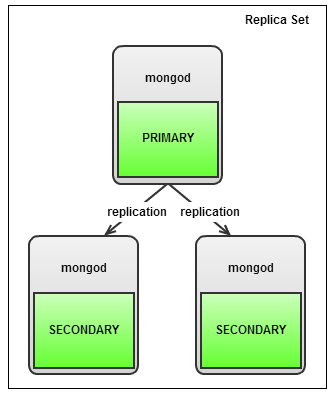
\includegraphics[scale=0.4]{figures/repset.png}
        \caption{Δομή ομάδας αντιγραφής}
        \label{replicaset}
    \end{figure}
    
    \item \selectlanguage{english}\textbf{Indexing --}\selectlanguage{greek} Τα πεδία σε μια \selectlanguage{english}MongoDB\selectlanguage{greek} βάση δεδομένων ακολουθούν μηδενική, πρωτοβάθμια ή δευτεροβάθμια δεικτοδότηση. Ο δείτκης αυτός αφορά την μοναδικότητα ή μη ενός πεδίου στη βάση.
    \item \selectlanguage{english}\textbf{Load balancing --}\selectlanguage{greek}  Η \selectlanguage{english}MongoDB\selectlanguage{greek} κλιμακώνεται οριζοντίως με τη χρήση της ιδιότητας τεμαχιοποίησης (\selectlanguage{english}sharding\selectlanguage{greek}). Ο χρήστης επιλέγει ένα ``\textit{κλειδί κοπής}'' (\selectlanguage{english}shard key\selectlanguage{greek}) το οποίο καθορίζει τον τρόπο κατανομής των δεδομένων μιας συλλογής. Τα δεδομένα χωρίζονται σε εύρη τιμών (με βάση το κλειδί αυτό) και κατανέμονται σε πολλαπλά \selectlanguage{english}shards\selectlanguage{greek} (ένα \selectlanguage{english}shard\selectlanguage{greek} είναι to κύριο έγγραφο και έχει ένα ή περισσότερα αντίγραφα). Εναλλακτικά, το κλειδί \selectlanguage{english}shard\selectlanguage{greek} μπορεί να κρυπτογραφηθεί μέσω \selectlanguage{english}hashing\selectlanguage{greek} για να χαρτογραφηθεί σε ένα \selectlanguage{english}shard\selectlanguage{greek} \textbf{--} επιτρέποντας μια ομοιόμορφη κατανομή δεδομένων. Η \selectlanguage{english}MongoDB\selectlanguage{greek} μπορεί να τρέξει σε πολλούς διακομιστές, εξισορροπώντας το φορτίο ή να αντιγράψει τα δεδομένα για να διατηρήσει το σύστημα σε λειτουργία και σε περίπτωση αποτυχίας υλικού \cite{[MONGO3]}.
     \item \selectlanguage{english}\textbf{File Storage --}\selectlanguage{greek}  Η \selectlanguage{english}MongoDB\selectlanguage{greek} μπορεί να χρησιμοποιηθεί ως σύστημα αρχείων, το οποίο ονομάζεται \selectlanguage{english}GridFS\selectlanguage{greek} \cite{[MONGO4]}, με δυνατότητες εξισορρόπησης φορτίου και αναπαραγωγής δεδομένων σε πολλαπλές μηχανές αποθήκευσης αρχείων. Το σύστημα \selectlanguage{english}GridFS\selectlanguage{greek} διαιρεί ένα αρχείο σε τμήματα, ή κομμάτια, και αποθηκεύει κάθε ένα από αυτά τα κομμάτια ως ξεχωριστό έγγραφο \cite{[MONGO5]}.
     \item \selectlanguage{english}\textbf{Aggregation --}\selectlanguage{greek}  Η \selectlanguage{english}MongoDB\selectlanguage{greek} διαθέτει τρεις μεθόδους συνάθροισης: του αγωγού συσσωμάτωσης (\selectlanguage{english}aggregation pipeline\selectlanguage{greek}), της άθροισης μέσω χαρτογράφησης (\selectlanguage{english}map-reduce function\selectlanguage{greek}) και τις μονού σκοπού μεθόδους συνάθροισης (\selectlanguage{english}single-purpose aggregation methods\selectlanguage{greek}) \cite{[MONGO6],[MONGO7]}.
\end{itemize}

Συμπερασματικά, η \selectlanguage{english}MongoDB\selectlanguage{greek} είναι σχεδιασμένη για να απλοποιήσει τη διαδικασία αποθήκευσης και αναζήτης δεδομένων. Δεν έχει συνθετες εντολές, αντιθέτως κάθε διαδικασία αναζήτησης είναι σαφής και σύντομη. Ο χρήστης παρέχει τις προϋποθέσεις ή τη συνθήκη που επιθυμεί και η \selectlanguage{english}MongoDB\selectlanguage{greek} επιστρέφει το αποτέλεσμα από τη βάση. Στην περίπτωση εύρεσης ενός εγγράφου κάνει συγκεκριμένη αναζήτηση, ενώ στην περίπτωση εύρεσης ενός πλήθους εγγράφων κάνει ομαδική αναζήτηση με σελιδοποίηση (\selectlanguage{english}pagination\selectlanguage{greek}). Η \selectlanguage{english}MongoDB\selectlanguage{greek}  είναι ευέλικτη και εύκολη στη χρήση, χάρις στην \selectlanguage{english}JSON\selectlanguage{greek} μορφοποίηση των δεδομένων, έναντι της χρήσης πικάνων (πχ. όπως στην \selectlanguage{english}SQL\selectlanguage{greek}). 


\subsection{Tαυτοποίηση Χρηστών (\selectlanguage{english}Open Authentication)}
\selectlanguage{greek}

Η ύπαρξη πολλών χρηστών σε μια εφαρμογή γεννά δύο βασικά προβλήματα. Το πρώτο συνίσταται από την ανάγκη διαχωρισμού των χρηστών μεταξύ τους, ενώ το δεύτερο έχει να κάνει με την παροχή προσωποποιημένων υπηρεσιών σε κάθε χρήστη. Σε αυτή την ενότητα γίνεται λόγος για τον τρόπο με τον οποίο επιλύονται τα παραπάνω προβλήματα. 

Οι εφαρμογές που δίνουν στους χρήστες τη δυνατότητα δημιουργίας προσωπικού λογαριασμού διαθέτουν ένα σύστημα επιβεβαίωσης και πρόσβασης εντός των υπηρεσιών τους. Το σύστημα αυτό ακολουθεί ένα πρωτόκολλο ταυτοποίησης γνωστό ως\selectlanguage{english} OAuth\selectlanguage{greek}.

\subsubsection{\selectlanguage{english}OAuth}
\selectlanguage{greek}

Το \selectlanguage{english}\textit{OAuth}\selectlanguage{greek} είναι ένα ανοιχτό πρότυπο το οποίο αναλαμβάνει την διαχείριση πρόσβασης στις υπηρεσίες μιας εφαρμογής από τους χρήστες της. Ο μηχανισμός αυτός χρησιμοποιείται σε όλες τις σημερινές εφαρμογές, όπως \selectlanguage{english}\textit{facebook, Microsoft, Google, Twitter, Amazon}\selectlanguage{greek} κλπ. Γενικά, το \selectlanguage{english}OAuth\selectlanguage{greek} παρέχει στους πελάτες μια ``\textit{ασφαλή εξουσιοδοτημένη πρόσβαση}'' σε πόρους ενός \selectlanguage{english}server\selectlanguage{greek} εξ' ονόματος του ιδιοκτήτη των πόρων αυτών. Καθορίζει μια διαδικασία εξουσιοδότησης πρόσβασης στους πόρους αυτούς σε τρίτους, χωρίς να μοιράζονται τα διαπιστευτήρια τους. Σχεδιασμένο ειδικά για να λειτουργεί με το πρωτόκολλο \selectlanguage{english}HTTP\selectlanguage{greek}, το \selectlanguage{english}OAuth\selectlanguage{greek} ουσιαστικά επιτρέπει την έκδοση πιστοποιητικών πρόσβασης σε πελάτες τρίτων μέσω ενός \selectlanguage{english}server\selectlanguage{greek} εξουσιοδότησης, με την έγκριση του ιδιοκτήτη πόρων. Το τρίτο μέρος χρησιμοποιεί το διακριτικό πρόσβασης για πρόσβαση στους προστατευόμενους πόρους που φιλοξενεί ο \selectlanguage{english}server\selectlanguage{greek} πόρων.

\subsubsection{\selectlanguage{english}Access Token}
\selectlanguage{greek}

Το σύμβολο πιστοποίησης (\selectlanguage{english}Access Token\selectlanguage{greek}) είναι ένα είδος πιστοποιητικού, το οποίο ένας πελάτης μπορεί να χρησιμοποιήσει για να αποκτήσει πρόσβαση σε προστατευμένους πόρους. Συγκεκριμένα είναι μία συμβολοσειρά χωρίς κάποια σημασία σε κανέναν εκτός από τον \selectlanguage{english}server\selectlanguage{greek}. Πέραν του ότι είναι μικρά σε μέγεθος και δεν προσθέτουν καθυστερήσεις, εμποδίζουν να χρησιμοποιούνται τα διαπεστευτήρια του ιδιοκτήτη (\selectlanguage{english}username, email, password\selectlanguage{greek}) συνεχώς και έτσι αν πέσει σε λάθος χέρια δεν τα αποκτά ο κακόβουλος χρήστης. Επιπλέον έχουν περιορισμένη πρόσβαση και συνήθως έχουν ημερομηνία λήξης, ώστε όταν αυτή παρέλθει, το σύμβολο αυτό παύει να ισχύει και δεν μπορεί να ξαναχρησιμοποιηθεί. Τότε, πρέπει να γίνει αίτηση για ανανέωση της ημερομηνίας (\selectlanguage{english}Refresh Token\selectlanguage{greek}).

Η διαδικασία ταυτοποίησης και έκδοσης \selectlanguage{english}access token\selectlanguage{greek} διακρίνεται σε τρία στάδια. Όταν ο χρήστης εισέρχεται για πρώτη φορά στην εφαρμογή, καλείται να δημιουργήσει λογαριασμό. Με αυτό τον τρόπο, ο χρήστης αποκτά πρόσβαση στους προστατευόμενους πόρους, καθώς επίσης και στις εξατομικευμένες εμπειρίες της εφαρμογής. Η είσοδος του χρήστη στην εφαρμογή γίνεται μέσω της συμπλήρωσης μιας φόρμας εγγραφής (\selectlanguage{english}register/signup form\selectlanguage{greek}). Η διαδικασία αυτή αποτελεί το πρώτο στάδιο. Αφού ο χρήστης χορηγήσει άδεια διαχείρισης των διαπιστευτηρίων του κάνοντας \selectlanguage{english}register\selectlanguage{greek} στην εφαρμογή, τότε μεταφέρεται αυτόματα εντός των υπηρεσιών της εφαρμογής. Κατά τη διάρεκεια της μετάβασης, ο \selectlanguage{english}server\selectlanguage{greek} είναι υπεύθυνος για την αποθήκευση των διαπιστευτηρίων του χρήστη και την ανταλλαγή (\selectlanguage{english}handshake\selectlanguage{greek}) τους με ένα μοναδικό \selectlanguage{english}access token\selectlanguage{greek} που αντιστοιχεί σε αυτόν τον χρήστη που μόλις πραγματοποίησε είσοδο στην εφαρμογή. Με άλλα λόγια, το \selectlanguage{english}access token\selectlanguage{greek} συμβολίζει το ``\textit{κλειδί}'' με το οποίο ο χρήστης ``\textit{ανοίγει}'' την εφαρμογή. Η ανταλλαγή αυτή αποτελεί το δεύτερο στάδιο.

Η διαδικασία αυτή είναι μονόδρομη, καθώς το πρώτο σταδιο αποτελεί απαραίτητη και αναγκαία συνθήκη για τη μετάβαση στο δεύτερο στάδιο. Ο χρήστης δεν μπορεί να παρακάμψει το πρώτο στάδιο καθώς η έκδοση \selectlanguage{english}access token\selectlanguage{greek} είναι υποχρεωτική για όλους τους χρήστες που επιθυμούν να καταναλώσουν τις υπηρεσίες τις εφαρμογής. Ωστόσο, μετά την έκδοση \selectlanguage{english}access token\selectlanguage{greek} ο χρήστης δεν χρειάζεται να επαναλάβει τη διαδικασία ταυτοποίησης. Εφόσον δεν πραγματοποιήσει έξοδο (\selectlanguage{english}logout\selectlanguage{greek}) από την εφαρμογή, έχει την δυνατότητα να «κλείσει» και να «ανοίξει» την εφαρμογή χωρίς την απαίτηση των διαπιστευτηρίων του. Το κλειδί αποθηκεύεται στη μνήμη της συσκευής για μελλοντική χρήση. Αυτό είναι και το νόημα της όλης διαδικασίας. Σε αυτή την περίπτωση, ο χρήστης κάνει είσοδο στην εφαρμογή παρακάμπτοντας το πρώτο στάδιο ταυτοποίησης, το οποίο γίνεται αυτόματα χάρις στο αποθηκευμένο κλειδί που είναι διαθέσιμο ασύγχρονα στην εφαρμογή. 

Για όσο διάστημα ο χρήστης έχει στη διάθεσή του κλειδί, μπορεί να είσερχεται στην εφαρμογή ή να εξέρχεται από αυτή κατ' επανάληψη. Αυτό οφείλεται στο γεγονός ότι ο χρήστης εξακολουθεί να είναι συνδεδεμένος. Ωστόσο, εάν για κάποιο λόγο ο χρήστης αποφασίσει να αποσυνδεθεί από την εφαρμογή κάνοντας \selectlanguage{english}logout\selectlanguage{greek}, τότε το \selectlanguage{english}access token\selectlanguage{greek} αφαιρείται και καταστρέφεται και ο χρήστης επαναφέρεται αυτόματα στην σελίδα εισόδου της εφαρμογής. Αυτή η διαδικασία αποτελεί το τρίτο και τελευταίο στάδιο, με το οποίο ολοκληρώνεται ο κύκλος ταυτοποίησης ενός χρήστη. Προκειμένου να αποκτηθεί εκ νέου πρόσβαση, πρέπει να επναληφθούν τα πρώτα δύο στάδια από την αρχή. Η μόνη διαφορά στην όλη διαδικασία είναι πως πλέον ο χρήστης είναι καταχωρημένος στη βάση της εφαρμογής και, επομένως δεν χρειάζεται να κάνει εκ νέου εγγραφή. Αρκεί να παρέχει τα διαπιστευτήριά του στην φόρμα εισόδου (\tl{login/signin form}) και στην περίπτωση επιτυχούς διασταύρωσης των στοιχείων, να συνδεθεί στο λογαριασμό του και να μεταφερθεί εντός της εφαρμογής.

\begin{figure}[h]
    \centering
    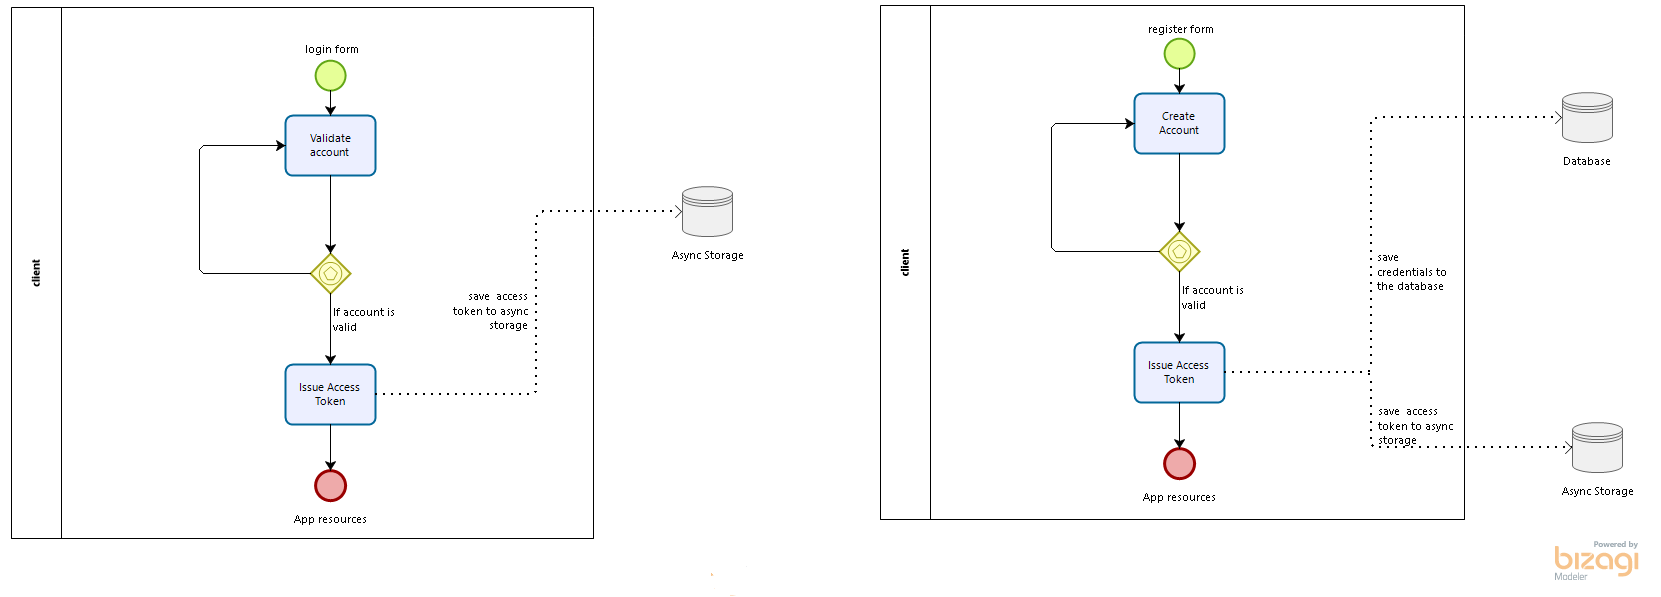
\includegraphics[scale=0.4]{figures/access-token.png}
    \caption{Διαδικασία έκδοσης \selectlanguage{english}access token\selectlanguage{greek}}
    \label{accesstoken}
\end{figure}


\subsubsection{\selectlanguage{english}JSON Web Token}
\selectlanguage{greek}

Το \selectlanguage{english}JWT\selectlanguage{greek} είναι μια μορφή \selectlanguage{english}access token\selectlanguage{greek} το οποίο εκδίδεται στην πλευρά του \selectlanguage{english}server\selectlanguage{greek} κατά την ταυτοποίηση ενός χρήστη. Κατά την επιτυχή είσοδο του χρήστη στην εφαρμογή, το \tl{JWT} αποθηκεύεται τοπικά στη μνήμη της συσκευής. Κάθε φορά που ο χρήστης θέλει να αποκτήσει πρόσβαση σε προστατευόμενους πόρους εντός της εφαρμογής, ανταλλάσσει το \selectlanguage{english}JWT\selectlanguage{greek} με τον προστατευόμενο πόρο μέσω μιας χειραψίας (\selectlanguage{english}handshake\selectlanguage{greek}). Η χειραψία είναι στην ουσία ένα αίτημα το οποίο αποστέλλεται στον \selectlanguage{english}server\selectlanguage{greek} και περιέχει, μεταξύ άλλων, και μια επικεφαλίδα εξουσιοδότησης (\selectlanguage{english}authorization header\selectlanguage{greek}). Το περιεχόμενο της επικεφαλίδας μοιάζει με το ακόλουθο:

\selectlanguage{english}
\begin{lstlisting}
Authorization: Bearer eyJhbGci...<snip>...yu5CSpyHI
\end{lstlisting}
\selectlanguage{greek}

Αυτός είναι ένας μηχανισμός ελέγχου ταυτότητας χωρίς κατάσταση, αφόυ η κατάσταση του χρήστη δεν αποθηκεύεται ποτέ στη μνήμη του \selectlanguage{english}server\selectlanguage{greek}. Οι προστατευμένες διαδρομές (\selectlanguage{english}routes\selectlanguage{greek}) του \selectlanguage{english}server\selectlanguage{greek} θα ελέγχουν την ύπαρξη έγκυρου \selectlanguage{english}JWT\selectlanguage{greek} στην επικεφαλίδα εξουσιοδότησης και, αν υπάρχει, ο χρήστης θα έχει πρόσβαση στους προστατευμένους πόρους. Καθώς τα \selectlanguage{english}JWTs\selectlanguage{greek} είναι αυτοτελή, υπάρχουν όλες οι απαραίτητες πληροφορίες, μειώνοντας την ανάγκη συχνών προσπελάσεων της βάσης δεδομένων \cite{[JWT1]}.

Τα βασικά πεδία που διαθέτει ένα \selectlanguage{english}JSON Web Token\selectlanguage{greek} φαίνονται στον κάτωθι πίνακα:


\begin{table}[h]
\centering
\begin{tabular}{ |m{2cm}|m{2cm}|m{8cm}|  }
\hline
\multicolumn{3}{|c|}{\selectlanguage{english}Standard JWT Fields\selectlanguage{greek}} \\
\hline 
\textit{\textbf{\selectlanguage{english}code\selectlanguage{greek}}} & \textit{\selectlanguage{english}\textbf{name}\selectlanguage{greek}} & \textit{\textbf{\selectlanguage{english}description\selectlanguage{greek}}}  \\
\hline 
\selectlanguage{english}\textit{iss} \selectlanguage{greek}
 & \selectlanguage{english}Issuer\selectlanguage{greek} & \selectlanguage{english}Identifies principal that issued the JWT.\\
\hline
\selectlanguage{english}\textit{sub} \selectlanguage{greek}
 & \selectlanguage{english}Subject\selectlanguage{greek} & \selectlanguage{english}Identifies the subject of the JWT.\\
\hline
\selectlanguage{english}\textit{aud} \selectlanguage{greek}
 & \selectlanguage{english}Audience\selectlanguage{greek} & \selectlanguage{english}Identifies the recipients that the JWT is intended for. Each principal intended to process the JWT \textbf{must} identify itself with a value in the audience claim. If the principal processing the claim does not identify itself with a value in the \textit{aud} claim when this claim is present, then the JWT \textbf{must} be rejected.\\
\hline
\selectlanguage{english}\textit{exp} \selectlanguage{greek}
 & \selectlanguage{english}Expiration Time\selectlanguage{greek} & \selectlanguage{english}Identifies the expiration time on and after which the JWT \textbf{must not} be accepted for processing. The value must be a \textit{NumericDate}: either an integer or decimal, representing seconds past \textit{1970-01-01 00:00:00Z.}\\
\hline
\selectlanguage{english}\textit{nbf} \selectlanguage{greek}
 & \selectlanguage{english}Not Before\selectlanguage{greek} & \selectlanguage{english}Identifies the time on which the JWT will start to be accepted for processing. The value must be a \textit{NumericDate}.\\
\hline
\selectlanguage{english}\textit{iat} \selectlanguage{greek}
 & \selectlanguage{english}Issued At\selectlanguage{greek} & \selectlanguage{english}Identifies the time at which the JWT was issued. The value must be a \textit{NumericDate}.\\
\hline
\selectlanguage{english}\textit{jti} \selectlanguage{greek}
 & \selectlanguage{english}JWT ID\selectlanguage{greek} & \selectlanguage{english}Case sensitive unique identifier of the token even among different issuers.\\
\hline
\end{tabular}
\selectlanguage{greek}
\caption{Δικαιώματα που μπορούν να αποδωθούν σε ένα \selectlanguage{english}JSON Web Token\selectlanguage{greek}}
\label{tab:parameters}
\end{table}



\subsubsection{\selectlanguage{english}Passport.js - Passport Strategies}
\selectlanguage{greek}

Για την ταυτοποίηση των χρηστών στην εφαρμογή χρησιμοποιήθηκε το λογισμικό \selectlanguage{english}Passport.js\selectlanguage{greek}. Το \selectlanguage{english}Passport\selectlanguage{greek} είναι ένα ενδιάμεσο λογισμικό το οποίο υλοποιείται σε \selectlanguage{english}JS\selectlanguage{greek} και υποστηρίζεται από τη \selectlanguage{english}Node.js\selectlanguage{greek}. Eίναι υπεύθυνο για την διαχείριση των χρηστών και την προστασία των πόρων της εφαρμογής. Συγκεκριμένα, πραγματοποιεί αναζήτηση στη βάση ενός χρήστη που επιχειρεί είσοδο στην εφαρμογή και σε περίπτωση επιτυχούς εύρεσης, εκδίδει \selectlanguage{english}token\selectlanguage{greek}.

Η προστασία των πόρων της εφαρμογής γίνεται με την υλοποίηση στατηγικών πακέτων (\selectlanguage{english}Strategies\selectlanguage{greek}) που διατίθενται από κατασκευής εντός της τεχνολογίας του \selectlanguage{english}Passport\selectlanguage{greek}. Στην εφαρμογή έγινε χρήση δύο εξ' αυτών:

\begin{itemize}
    \item \selectlanguage{english}\textbf{JWT Strategy}\selectlanguage{greek}
    \item \selectlanguage{english}\textbf{Local Strategy}\selectlanguage{greek}
\end{itemize}

Η \selectlanguage{english}JWT Strategy\selectlanguage{greek} αναλαμβάνει την προστασία των πόρων της εφαρμογής από μη εγγεγραμμένους χρήστες. Αυτό επιτυγχάνεται με τον έλεγχο κάθε φορά που γίνεται αίτημα της επικεφαλίδας εξουσιοδότητης. Εάν αυτή φέρει κάποιο \selectlanguage{english}token\selectlanguage{greek} τότε επιτρέπεται η πρόσβαση στους ζητούμενους πόρους. Αυτή η διαδικασία αποτελεί το αντίστροφο της χειραψίας που αναφέρθηκε νωρίτερα μεταξύ \selectlanguage{english}client-server\selectlanguage{greek}.

Η \selectlanguage{english}Local Strategy\selectlanguage{greek} είναι υπεύθυνη για τη διαδικασία εγγραφής ή σύνδεσης των χρηστών στην εφαρμογή. Με την υποβολή της αίτησης για δημιουργία λογαριασμού στην εφαρμογή από ένα νέο χρήστη, τα στοιχεία αποστέλλονται προς αποθήκευση στη βάση. Στην περίπτωση που η διαδικασία εγγραφής ολοκληρωθεί επιτυχώς (ο συνδυασμός των διαπιστευτηρίων του χρήστη πρέπει να είναι μοναδικός), τότε το \selectlanguage{english}Passport\selectlanguage{greek} εκδίδει \selectlanguage{english}token\selectlanguage{greek} για το νέο χρήστη και εκείνος αποκτά πρόσβαση στους πόρους της εφαρμογής. Αντιστοίχως, όταν ένας ήδη υπάρχων χρήστης κάνει αίτηση για σύνδεση στο λογαριασμό του, τότε γίνεται ο κατάλληλος έλεγχος στον συνδυασμό των διαπιστευτηρίων του, και σε περίπτωση επιτυχίας εκδίδεται νέο \selectlanguage{english}token\selectlanguage{greek} για τον χρήστη αυτό. 

\selectlanguage{english}
\begin{lstlisting}[language=JavaScript, caption=\selectlanguage{greek}Βασικό \selectlanguage{english}boilerplate\selectlanguage{greek} της \selectlanguage{english}Local Strategy\selectlanguage{greek} στην εφαρμογή]
passport.use(new LocalStrategy(
  function(username, password, done) {
    User.findOne({ username: username }, function (err, user) {
      if (err) { return done(err); }
      if (!user) { return done(null, false); }
      if (!user.verifyPassword(password)) { return done(null, false); }
      return done(null, user);
    });
  }
));
\end{lstlisting}
\selectlanguage{greek}
=======


\end{lstlisting}



\subsection{\selectlanguage{english}JavaScript}
\selectlanguage{greek}
Μιλαμε εισαγωγικα για τη γλωσσα αυτη, ιδεες απο τη διπλωματικη του παιδιου και περναμε στην Ρεακτ. Μιλαμε για τα γνωρισματα και τα πλεονεκτηματα της (παρε την περιληψη που εγραψες).

\subsubsection{\selectlanguage{english}React Native}

>>>>>>> acacc83a12cc6f1be99d6d3fb0df8b0ed3fa708b
